\documentclass{article}
\usepackage[a4paper,landscape,margin=1.5cm]{geometry}
\usepackage{pgfplots}
\pgfplotsset{compat=1.18}
\pagestyle{empty}
\begin{document}
\section*{\texttt{cnot/A-measured-by-order.tex}}
Suzuki formulas of each order, r from: Measured $r$; median over seeds, bars min-max\par\medskip
% Generated by pysimcount.pfseeds -- do not edit; regenerate instead.
% figure: A-measured-by-order -- Suzuki formulas of each order, r from: Measured $r$; median over seeds [1, 2, 3, 4, 5, 6, 7, 8, 9, 10], bars = min..max
% metric=cnot gatebase=cz merged
% seed 1: git_commit=01d3c275ceae2840002bd1aaea68f59b987c4975 git_dirty=False
% seed 2: git_commit=01d3c275ceae2840002bd1aaea68f59b987c4975 git_dirty=False
% seed 3: git_commit=01d3c275ceae2840002bd1aaea68f59b987c4975 git_dirty=False
% seed 4: git_commit=01d3c275ceae2840002bd1aaea68f59b987c4975 git_dirty=False
% seed 5: git_commit=01d3c275ceae2840002bd1aaea68f59b987c4975 git_dirty=False
% seed 6: git_commit=01d3c275ceae2840002bd1aaea68f59b987c4975 git_dirty=False
% seed 7: git_commit=01d3c275ceae2840002bd1aaea68f59b987c4975 git_dirty=False
% seed 8: git_commit=01d3c275ceae2840002bd1aaea68f59b987c4975 git_dirty=False
% seed 9: git_commit=01d3c275ceae2840002bd1aaea68f59b987c4975 git_dirty=False
% seed 10: git_commit=01d3c275ceae2840002bd1aaea68f59b987c4975 git_dirty=False
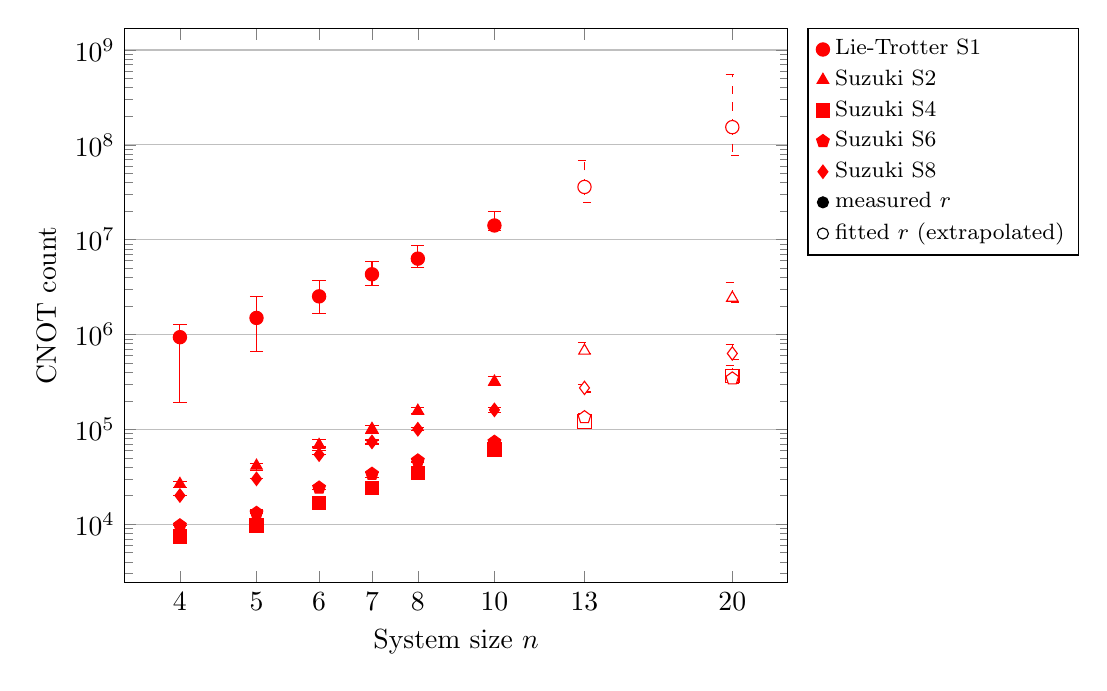
\begin{tikzpicture}
  \begin{loglogaxis}[
    width=10cm,
    xlabel={System size $n$},
    ylabel={CNOT count},
    xtick={4,5,6,7,8,10,13,20},
    xticklabels={4,5,6,7,8,10,13,20},
    ymajorgrids=true,
    legend pos=outer north east,
    legend cell align=left,
    legend style={font=\footnotesize},
  ]
    \addplot[only marks, red, mark=*, mark size=2.4pt, mark options={solid, fill=red}, error bars/.cd, y dir=both, y explicit, error bar style={red}] coordinates {
      (4,937416) += (0,325728) -= (0,745032)
      (5,1495575) += (0,1023825) -= (0,830775)
      (6,2525040) += (0,1222236) -= (0,866160)
      (7,4318944) += (0,1528632) -= (0,1003338)
      (8,6310224) += (0,2439408) -= (0,1227024)
      (10,14120670) += (0,5649510) -= (0,1722750)
    };
    \addlegendentry{Lie-Trotter S1}
    \addplot[only marks, red, mark=*, mark size=2.4pt, mark options={solid, fill=white}, forget plot, error bars/.cd, y dir=both, y explicit, error bar style={red, dashed}] coordinates {
      (13,35981283) += (0,33058077) -= (0,11393655)
      (20,153747180) += (0,399150900) -= (0,76118820)
    };
    \addplot[only marks, red, mark=triangle*, mark size=2.4pt, mark options={solid, fill=red}, error bars/.cd, y dir=both, y explicit, error bar style={red}] coordinates {
      (4,26460) += (0,1500) -= (0,2300)
      (5,41200) += (0,2750) -= (0,4250)
      (6,68250) += (0,10230) -= (0,3150)
      (7,100765) += (0,9555) -= (0,10955)
      (8,156440) += (0,13400) -= (0,8360)
      (10,317650) += (0,43350) -= (0,26450)
    };
    \addlegendentry{Suzuki S2}
    \addplot[only marks, red, mark=triangle*, mark size=2.4pt, mark options={solid, fill=white}, forget plot, error bars/.cd, y dir=both, y explicit, error bar style={red, dashed}] coordinates {
      (13,673790) += (0,149630) -= (0,46410)
      (20,2428200) += (0,1074200) -= (0,230000)
    };
    \addplot[only marks, red, mark=square*, mark size=2.4pt, mark options={solid, fill=red}, error bars/.cd, y dir=both, y explicit, error bar style={red}] coordinates {
      (4,7392) += (0,168) -= (0,0)
      (5,9660) += (0,420) -= (0,210)
      (6,16632) += (0,1260) -= (0,756)
      (7,23961) += (0,2205) -= (0,1323)
      (8,34608) += (0,1344) -= (0,1344)
      (10,61530) += (0,5670) -= (0,1470)
    };
    \addlegendentry{Suzuki S4}
    \addplot[only marks, red, mark=square*, mark size=2.4pt, mark options={solid, fill=white}, forget plot, error bars/.cd, y dir=both, y explicit, error bar style={red, dashed}] coordinates {
      (13,120939) += (0,17199) -= (0,7917)
      (20,363720) += (0,102480) -= (0,42000)
    };
    \addplot[only marks, red, mark=pentagon*, mark size=2.4pt, mark options={solid, fill=red}, error bars/.cd, y dir=both, y explicit, error bar style={red}] coordinates {
      (4,9696) += (0,0) -= (0,0)
      (5,13130) += (0,1010) -= (0,0)
      (6,24240) += (0,1212) -= (0,1212)
      (7,33936) += (0,1414) -= (0,2828)
      (8,46864) += (0,1616) -= (0,1616)
      (10,73730) += (0,5050) -= (0,3030)
    };
    \addlegendentry{Suzuki S6}
    \addplot[only marks, red, mark=pentagon*, mark size=2.4pt, mark options={solid, fill=white}, forget plot, error bars/.cd, y dir=both, y explicit, error bar style={red, dashed}] coordinates {
      (13,133926) += (0,13130) -= (0,7878)
      (20,343400) += (0,68680) -= (0,36360)
    };
    \addplot[only marks, red, mark=diamond*, mark size=2.4pt, mark options={solid, fill=red}, error bars/.cd, y dir=both, y explicit, error bar style={red}] coordinates {
      (4,20040) += (0,0) -= (0,0)
      (5,30060) += (0,0) -= (0,0)
      (6,54108) += (0,6012) -= (0,0)
      (7,73647) += (0,3507) -= (0,3507)
      (8,100200) += (0,4008) -= (0,4008)
      (10,160320) += (0,10020) -= (0,10020)
    };
    \addlegendentry{Suzuki S8}
    \addplot[only marks, red, mark=diamond*, mark size=2.4pt, mark options={solid, fill=white}, forget plot, error bars/.cd, y dir=both, y explicit, error bar style={red, dashed}] coordinates {
      (13,273546) += (0,26052) -= (0,26052)
      (20,631260) += (0,150300) -= (0,90180)
    };
    \addlegendimage{only marks, black, mark=*}
    \addlegendentry{measured $r$}
    \addlegendimage{only marks, black, mark=*, mark options={fill=white}}
    \addlegendentry{fitted $r$ (extrapolated)}
  \end{loglogaxis}
\end{tikzpicture}

\clearpage

\section*{\texttt{cnot/B-order4-by-formula.tex}}
Every order-4 formula at measured r; median over seeds, bars min-max\par\medskip
% Generated by pysimcount.pfseeds -- do not edit; regenerate instead.
% figure: B-order4-by-formula -- Every order-4 formula at measured r; median over seeds [1, 2, 3, 4, 5, 6, 7, 8, 9, 10], bars = min..max
% metric=cnot gatebase=cz merged
% seed 1: git_commit=01d3c275ceae2840002bd1aaea68f59b987c4975 git_dirty=False
% seed 2: git_commit=01d3c275ceae2840002bd1aaea68f59b987c4975 git_dirty=False
% seed 3: git_commit=01d3c275ceae2840002bd1aaea68f59b987c4975 git_dirty=False
% seed 4: git_commit=01d3c275ceae2840002bd1aaea68f59b987c4975 git_dirty=False
% seed 5: git_commit=01d3c275ceae2840002bd1aaea68f59b987c4975 git_dirty=False
% seed 6: git_commit=01d3c275ceae2840002bd1aaea68f59b987c4975 git_dirty=False
% seed 7: git_commit=01d3c275ceae2840002bd1aaea68f59b987c4975 git_dirty=False
% seed 8: git_commit=01d3c275ceae2840002bd1aaea68f59b987c4975 git_dirty=False
% seed 9: git_commit=01d3c275ceae2840002bd1aaea68f59b987c4975 git_dirty=False
% seed 10: git_commit=01d3c275ceae2840002bd1aaea68f59b987c4975 git_dirty=False
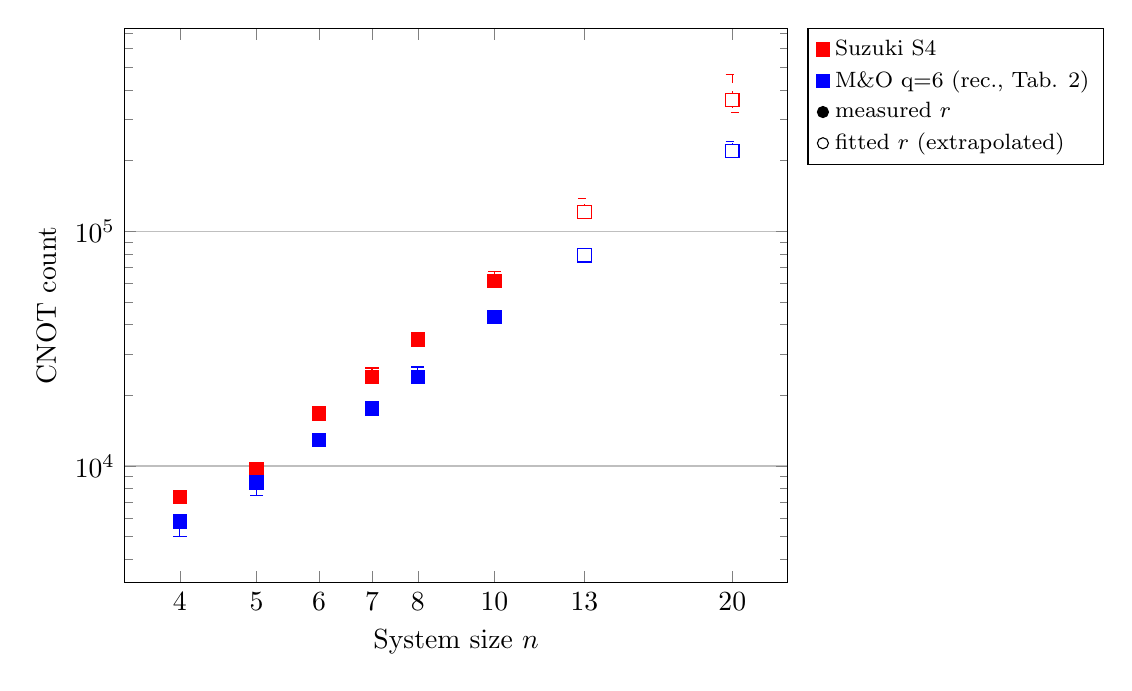
\begin{tikzpicture}
  \begin{loglogaxis}[
    width=10cm,
    xlabel={System size $n$},
    ylabel={CNOT count},
    xtick={4,5,6,7,8,10,13,20},
    xticklabels={4,5,6,7,8,10,13,20},
    ymajorgrids=true,
    legend pos=outer north east,
    legend cell align=left,
    legend style={font=\footnotesize},
  ]
    \addplot[only marks, red, mark=square*, mark size=2.4pt, mark options={solid, fill=red}, error bars/.cd, y dir=both, y explicit, error bar style={red}] coordinates {
      (4,7392) += (0,168) -= (0,0)
      (5,9660) += (0,420) -= (0,210)
      (6,16632) += (0,1260) -= (0,756)
      (7,23961) += (0,2205) -= (0,1323)
      (8,34608) += (0,1344) -= (0,1344)
      (10,61530) += (0,5670) -= (0,1470)
    };
    \addlegendentry{Suzuki S4}
    \addplot[only marks, red, mark=square*, mark size=2.4pt, mark options={solid, fill=white}, forget plot, error bars/.cd, y dir=both, y explicit, error bar style={red, dashed}] coordinates {
      (13,120939) += (0,17199) -= (0,7917)
      (20,363720) += (0,102480) -= (0,42000)
    };
    \addplot[only marks, blue, mark=square*, mark size=2.4pt, mark options={solid, fill=blue}, error bars/.cd, y dir=both, y explicit, error bar style={blue}] coordinates {
      (4,5800) += (0,200) -= (0,800)
      (5,8500) += (0,250) -= (0,1000)
      (6,12900) += (0,300) -= (0,600)
      (7,17675) += (0,875) -= (0,1225)
      (8,24000) += (0,2400) -= (0,1200)
      (10,43250) += (0,1750) -= (0,2750)
    };
    \addlegendentry{M\&O q=6 (rec., Tab. 2)}
    \addplot[only marks, blue, mark=square*, mark size=2.4pt, mark options={solid, fill=white}, forget plot, error bars/.cd, y dir=both, y explicit, error bar style={blue, dashed}] coordinates {
      (13,78975) += (0,5525) -= (0,1625)
      (20,219500) += (0,21500) -= (0,8500)
    };
    \addlegendimage{only marks, black, mark=*}
    \addlegendentry{measured $r$}
    \addlegendimage{only marks, black, mark=*, mark options={fill=white}}
    \addlegendentry{fitted $r$ (extrapolated)}
  \end{loglogaxis}
\end{tikzpicture}

\clearpage

\section*{\texttt{cnot/B-order6-by-formula.tex}}
Every order-6 formula at measured r; median over seeds, bars min-max\par\medskip
% Generated by pysimcount.pfseeds -- do not edit; regenerate instead.
% figure: B-order6-by-formula -- Every order-6 formula at measured r; median over seeds [1, 2, 3, 4, 5, 6, 7, 8, 9, 10], bars = min..max
% metric=cnot gatebase=cz merged
% seed 1: git_commit=01d3c275ceae2840002bd1aaea68f59b987c4975 git_dirty=False
% seed 2: git_commit=01d3c275ceae2840002bd1aaea68f59b987c4975 git_dirty=False
% seed 3: git_commit=01d3c275ceae2840002bd1aaea68f59b987c4975 git_dirty=False
% seed 4: git_commit=01d3c275ceae2840002bd1aaea68f59b987c4975 git_dirty=False
% seed 5: git_commit=01d3c275ceae2840002bd1aaea68f59b987c4975 git_dirty=False
% seed 6: git_commit=01d3c275ceae2840002bd1aaea68f59b987c4975 git_dirty=False
% seed 7: git_commit=01d3c275ceae2840002bd1aaea68f59b987c4975 git_dirty=False
% seed 8: git_commit=01d3c275ceae2840002bd1aaea68f59b987c4975 git_dirty=False
% seed 9: git_commit=01d3c275ceae2840002bd1aaea68f59b987c4975 git_dirty=False
% seed 10: git_commit=01d3c275ceae2840002bd1aaea68f59b987c4975 git_dirty=False
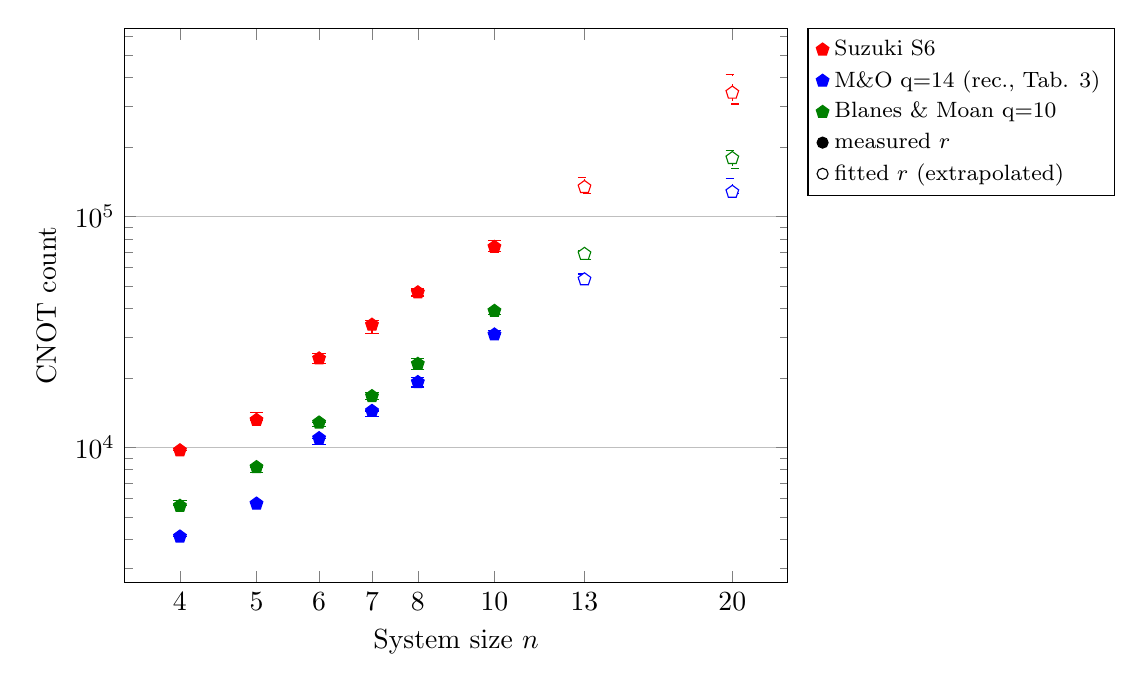
\begin{tikzpicture}
  \begin{loglogaxis}[
    width=10cm,
    xlabel={System size $n$},
    ylabel={CNOT count},
    xtick={4,5,6,7,8,10,13,20},
    xticklabels={4,5,6,7,8,10,13,20},
    ymajorgrids=true,
    legend pos=outer north east,
    legend cell align=left,
    legend style={font=\footnotesize},
  ]
    \addplot[only marks, red, mark=pentagon*, mark size=2.4pt, mark options={solid, fill=red}, error bars/.cd, y dir=both, y explicit, error bar style={red}] coordinates {
      (4,9696) += (0,0) -= (0,0)
      (5,13130) += (0,1010) -= (0,0)
      (6,24240) += (0,1212) -= (0,1212)
      (7,33936) += (0,1414) -= (0,2828)
      (8,46864) += (0,1616) -= (0,1616)
      (10,73730) += (0,5050) -= (0,3030)
    };
    \addlegendentry{Suzuki S6}
    \addplot[only marks, red, mark=pentagon*, mark size=2.4pt, mark options={solid, fill=white}, forget plot, error bars/.cd, y dir=both, y explicit, error bar style={red, dashed}] coordinates {
      (13,133926) += (0,13130) -= (0,7878)
      (20,343400) += (0,68680) -= (0,36360)
    };
    \addplot[only marks, blue, mark=pentagon*, mark size=2.4pt, mark options={solid, fill=blue}, error bars/.cd, y dir=both, y explicit, error bar style={blue}] coordinates {
      (4,4104) += (0,0) -= (0,0)
      (5,5700) += (0,0) -= (0,0)
      (6,10944) += (0,0) -= (0,684)
      (7,14364) += (0,0) -= (0,798)
      (8,19152) += (0,912) -= (0,912)
      (10,30780) += (0,1140) -= (0,0)
    };
    \addlegendentry{M\&O q=14 (rec., Tab. 3)}
    \addplot[only marks, blue, mark=pentagon*, mark size=2.4pt, mark options={solid, fill=white}, forget plot, error bars/.cd, y dir=both, y explicit, error bar style={blue, dashed}] coordinates {
      (13,53352) += (0,2964) -= (0,0)
      (20,127680) += (0,18240) -= (0,2280)
    };
    \addplot[only marks, green!50!black, mark=pentagon*, mark size=2.4pt, mark options={solid, fill=green!50!black}, error bars/.cd, y dir=both, y explicit, error bar style={green!50!black}] coordinates {
      (4,5576) += (0,328) -= (0,0)
      (5,8200) += (0,0) -= (0,410)
      (6,12792) += (0,0) -= (0,492)
      (7,16646) += (0,574) -= (0,574)
      (8,22960) += (0,1312) -= (0,1312)
      (10,38950) += (0,410) -= (0,1230)
    };
    \addlegendentry{Blanes \& Moan q=10}
    \addplot[only marks, green!50!black, mark=pentagon*, mark size=2.4pt, mark options={solid, fill=white}, forget plot, error bars/.cd, y dir=both, y explicit, error bar style={green!50!black, dashed}] coordinates {
      (13,68757) += (0,2665) -= (0,3731)
      (20,178760) += (0,14760) -= (0,18040)
    };
    \addlegendimage{only marks, black, mark=*}
    \addlegendentry{measured $r$}
    \addlegendimage{only marks, black, mark=*, mark options={fill=white}}
    \addlegendentry{fitted $r$ (extrapolated)}
  \end{loglogaxis}
\end{tikzpicture}

\clearpage

\section*{\texttt{cnot/B-order8-by-formula.tex}}
Every order-8 formula at measured r; median over seeds, bars min-max\par\medskip
% Generated by plsimcount.pfseeds -- do not edit; regenerate instead.
% figure: B-order8-by-formula -- Every order-8 formula at measured r; median over seeds [1, 2, 3, 4, 5, 6, 7, 8, 9, 10], bars = min..max
% metric=cnot gatebase=cz merged
% seed 1: git_commit=01d3c275ceae2840002bd1aaea68f59b987c4975 git_dirty=False
% seed 2: git_commit=01d3c275ceae2840002bd1aaea68f59b987c4975 git_dirty=False
% seed 3: git_commit=01d3c275ceae2840002bd1aaea68f59b987c4975 git_dirty=False
% seed 4: git_commit=01d3c275ceae2840002bd1aaea68f59b987c4975 git_dirty=False
% seed 5: git_commit=01d3c275ceae2840002bd1aaea68f59b987c4975 git_dirty=False
% seed 6: git_commit=01d3c275ceae2840002bd1aaea68f59b987c4975 git_dirty=False
% seed 7: git_commit=01d3c275ceae2840002bd1aaea68f59b987c4975 git_dirty=False
% seed 8: git_commit=01d3c275ceae2840002bd1aaea68f59b987c4975 git_dirty=False
% seed 9: git_commit=01d3c275ceae2840002bd1aaea68f59b987c4975 git_dirty=False
% seed 10: git_commit=01d3c275ceae2840002bd1aaea68f59b987c4975 git_dirty=False
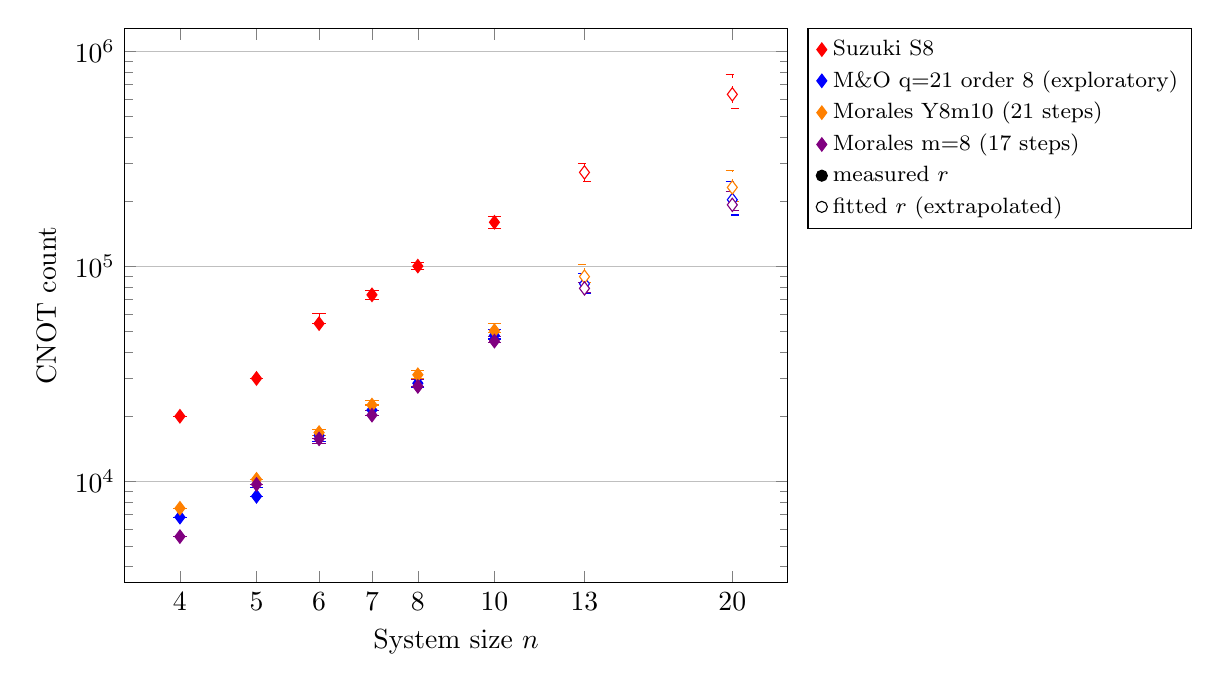
\begin{tikzpicture}
  \begin{loglogaxis}[
    width=10cm,
    xlabel={System size $n$},
    ylabel={CNOT count},
    xtick={4,5,6,7,8,10,13,20},
    xticklabels={4,5,6,7,8,10,13,20},
    ymajorgrids=true,
    legend pos=outer north east,
    legend cell align=left,
    legend style={font=\footnotesize},
  ]
    \addplot[only marks, red, mark=diamond*, mark size=2.4pt, mark options={solid, fill=red}, error bars/.cd, y dir=both, y explicit, error bar style={red}] coordinates {
      (4,20040) += (0,0) -= (0,0)
      (5,30060) += (0,0) -= (0,0)
      (6,54108) += (0,6012) -= (0,0)
      (7,73647) += (0,3507) -= (0,3507)
      (8,100200) += (0,4008) -= (0,4008)
      (10,160320) += (0,10020) -= (0,10020)
    };
    \addlegendentry{Suzuki S8}
    \addplot[only marks, red, mark=diamond*, mark size=2.4pt, mark options={solid, fill=white}, forget plot, error bars/.cd, y dir=both, y explicit, error bar style={red, dashed}] coordinates {
      (13,273546) += (0,26052) -= (0,26052)
      (20,631260) += (0,150300) -= (0,90180)
    };
    \addplot[only marks, blue, mark=diamond*, mark size=2.4pt, mark options={solid, fill=blue}, error bars/.cd, y dir=both, y explicit, error bar style={blue}] coordinates {
      (4,6800) += (0,0) -= (0,0)
      (5,8500) += (0,850) -= (0,0)
      (6,16320) += (0,1020) -= (0,1020)
      (7,21420) += (0,1190) -= (0,1190)
      (8,28560) += (0,1360) -= (0,1360)
      (10,47600) += (0,3400) -= (0,1700)
    };
    \addlegendentry{M\&O q=21 order 8 (exploratory)}
    \addplot[only marks, blue, mark=diamond*, mark size=2.4pt, mark options={solid, fill=white}, forget plot, error bars/.cd, y dir=both, y explicit, error bar style={blue, dashed}] coordinates {
      (13,82875) += (0,9945) -= (0,7735)
      (20,204000) += (0,44200) -= (0,30600)
    };
    \addplot[only marks, orange, mark=diamond*, mark size=2.4pt, mark options={solid, fill=orange}, error bars/.cd, y dir=both, y explicit, error bar style={orange}] coordinates {
      (4,7480) += (0,0) -= (0,0)
      (5,10200) += (0,0) -= (0,0)
      (6,16830) += (0,510) -= (0,510)
      (7,22610) += (0,1190) -= (0,0)
      (8,31280) += (0,1360) -= (0,1360)
      (10,50150) += (0,4250) -= (0,850)
    };
    \addlegendentry{Morales Y8m10 (21 steps)}
    \addplot[only marks, orange, mark=diamond*, mark size=2.4pt, mark options={solid, fill=white}, forget plot, error bars/.cd, y dir=both, y explicit, error bar style={orange, dashed}] coordinates {
      (13,89505) += (0,12155) -= (0,5525)
      (20,232900) += (0,45900) -= (0,32300)
    };
    \addplot[only marks, violet, mark=diamond*, mark size=2.4pt, mark options={solid, fill=violet}, error bars/.cd, y dir=both, y explicit, error bar style={violet}] coordinates {
      (4,5520) += (0,0) -= (0,0)
      (5,9660) += (0,0) -= (0,0)
      (6,15732) += (0,0) -= (0,828)
      (7,20286) += (0,966) -= (0,0)
      (8,27600) += (0,2208) -= (0,0)
      (10,44850) += (0,2070) -= (0,690)
    };
    \addlegendentry{Morales m=8 (17 steps)}
    \addplot[only marks, violet, mark=diamond*, mark size=2.4pt, mark options={solid, fill=white}, forget plot, error bars/.cd, y dir=both, y explicit, error bar style={violet, dashed}] coordinates {
      (13,78936) += (0,5382) -= (0,3588)
      (20,193200) += (0,30360) -= (0,11040)
    };
    \addlegendimage{only marks, black, mark=*}
    \addlegendentry{measured $r$}
    \addlegendimage{only marks, black, mark=*, mark options={fill=white}}
    \addlegendentry{fitted $r$ (extrapolated)}
  \end{loglogaxis}
\end{tikzpicture}

\clearpage

\section*{\texttt{cnot/B-all-by-formula.tex}}
Every formula at measured r; median over seeds, bars min-max\par\medskip
% Generated by plsimcount.pfseeds -- do not edit; regenerate instead.
% figure: B-all-by-formula -- Every formula at measured r; median over seeds [1, 2, 3, 4, 5, 6, 7, 8, 9, 10], bars = min..max
% metric=cnot gatebase=cz merged
% seed 1: git_commit=01d3c275ceae2840002bd1aaea68f59b987c4975 git_dirty=False
% seed 2: git_commit=01d3c275ceae2840002bd1aaea68f59b987c4975 git_dirty=False
% seed 3: git_commit=01d3c275ceae2840002bd1aaea68f59b987c4975 git_dirty=False
% seed 4: git_commit=01d3c275ceae2840002bd1aaea68f59b987c4975 git_dirty=False
% seed 5: git_commit=01d3c275ceae2840002bd1aaea68f59b987c4975 git_dirty=False
% seed 6: git_commit=01d3c275ceae2840002bd1aaea68f59b987c4975 git_dirty=False
% seed 7: git_commit=01d3c275ceae2840002bd1aaea68f59b987c4975 git_dirty=False
% seed 8: git_commit=01d3c275ceae2840002bd1aaea68f59b987c4975 git_dirty=False
% seed 9: git_commit=01d3c275ceae2840002bd1aaea68f59b987c4975 git_dirty=False
% seed 10: git_commit=01d3c275ceae2840002bd1aaea68f59b987c4975 git_dirty=False
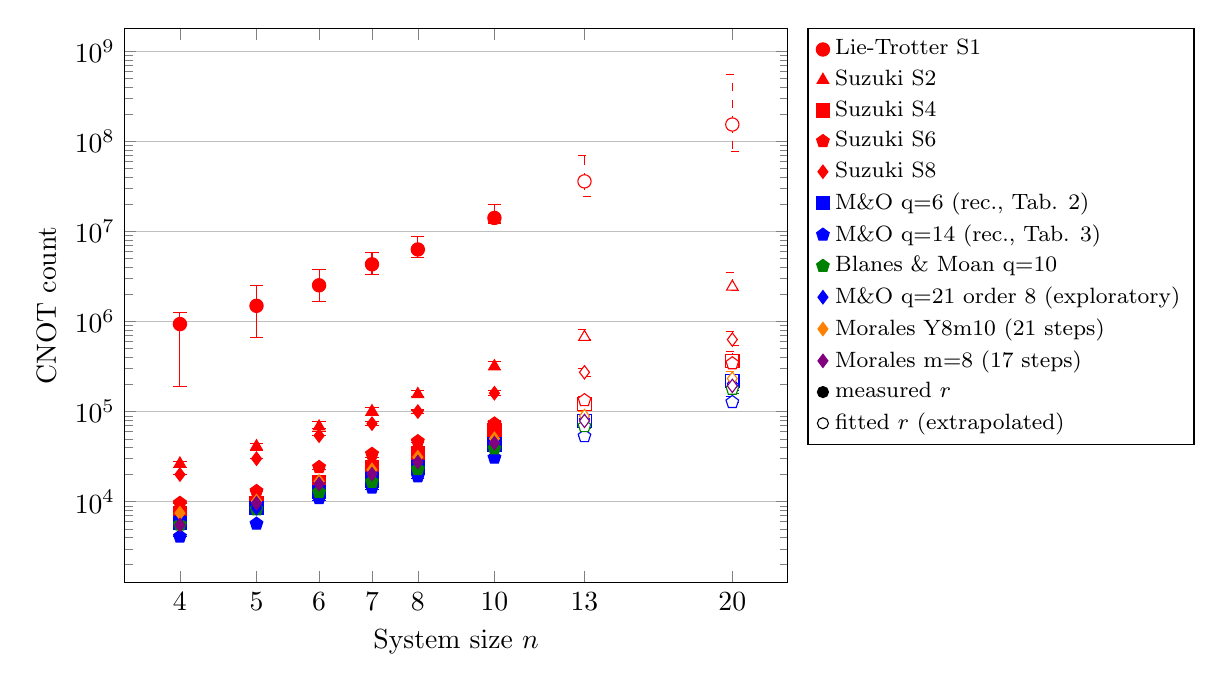
\begin{tikzpicture}
  \begin{loglogaxis}[
    width=10cm,
    xlabel={System size $n$},
    ylabel={CNOT count},
    xtick={4,5,6,7,8,10,13,20},
    xticklabels={4,5,6,7,8,10,13,20},
    ymajorgrids=true,
    legend pos=outer north east,
    legend cell align=left,
    legend style={font=\footnotesize},
  ]
    \addplot[only marks, red, mark=*, mark size=2.4pt, mark options={solid, fill=red}, error bars/.cd, y dir=both, y explicit, error bar style={red}] coordinates {
      (4,937416) += (0,325728) -= (0,745032)
      (5,1495575) += (0,1023825) -= (0,830775)
      (6,2525040) += (0,1222236) -= (0,866160)
      (7,4318944) += (0,1528632) -= (0,1003338)
      (8,6310224) += (0,2439408) -= (0,1227024)
      (10,14120670) += (0,5649510) -= (0,1722750)
    };
    \addlegendentry{Lie-Trotter S1}
    \addplot[only marks, red, mark=*, mark size=2.4pt, mark options={solid, fill=white}, forget plot, error bars/.cd, y dir=both, y explicit, error bar style={red, dashed}] coordinates {
      (13,35981283) += (0,33058077) -= (0,11393655)
      (20,153747180) += (0,399150900) -= (0,76118820)
    };
    \addplot[only marks, red, mark=triangle*, mark size=2.4pt, mark options={solid, fill=red}, error bars/.cd, y dir=both, y explicit, error bar style={red}] coordinates {
      (4,26460) += (0,1500) -= (0,2300)
      (5,41200) += (0,2750) -= (0,4250)
      (6,68250) += (0,10230) -= (0,3150)
      (7,100765) += (0,9555) -= (0,10955)
      (8,156440) += (0,13400) -= (0,8360)
      (10,317650) += (0,43350) -= (0,26450)
    };
    \addlegendentry{Suzuki S2}
    \addplot[only marks, red, mark=triangle*, mark size=2.4pt, mark options={solid, fill=white}, forget plot, error bars/.cd, y dir=both, y explicit, error bar style={red, dashed}] coordinates {
      (13,673790) += (0,149630) -= (0,46410)
      (20,2428200) += (0,1074200) -= (0,230000)
    };
    \addplot[only marks, red, mark=square*, mark size=2.4pt, mark options={solid, fill=red}, error bars/.cd, y dir=both, y explicit, error bar style={red}] coordinates {
      (4,7392) += (0,168) -= (0,0)
      (5,9660) += (0,420) -= (0,210)
      (6,16632) += (0,1260) -= (0,756)
      (7,23961) += (0,2205) -= (0,1323)
      (8,34608) += (0,1344) -= (0,1344)
      (10,61530) += (0,5670) -= (0,1470)
    };
    \addlegendentry{Suzuki S4}
    \addplot[only marks, red, mark=square*, mark size=2.4pt, mark options={solid, fill=white}, forget plot, error bars/.cd, y dir=both, y explicit, error bar style={red, dashed}] coordinates {
      (13,120939) += (0,17199) -= (0,7917)
      (20,363720) += (0,102480) -= (0,42000)
    };
    \addplot[only marks, red, mark=pentagon*, mark size=2.4pt, mark options={solid, fill=red}, error bars/.cd, y dir=both, y explicit, error bar style={red}] coordinates {
      (4,9696) += (0,0) -= (0,0)
      (5,13130) += (0,1010) -= (0,0)
      (6,24240) += (0,1212) -= (0,1212)
      (7,33936) += (0,1414) -= (0,2828)
      (8,46864) += (0,1616) -= (0,1616)
      (10,73730) += (0,5050) -= (0,3030)
    };
    \addlegendentry{Suzuki S6}
    \addplot[only marks, red, mark=pentagon*, mark size=2.4pt, mark options={solid, fill=white}, forget plot, error bars/.cd, y dir=both, y explicit, error bar style={red, dashed}] coordinates {
      (13,133926) += (0,13130) -= (0,7878)
      (20,343400) += (0,68680) -= (0,36360)
    };
    \addplot[only marks, red, mark=diamond*, mark size=2.4pt, mark options={solid, fill=red}, error bars/.cd, y dir=both, y explicit, error bar style={red}] coordinates {
      (4,20040) += (0,0) -= (0,0)
      (5,30060) += (0,0) -= (0,0)
      (6,54108) += (0,6012) -= (0,0)
      (7,73647) += (0,3507) -= (0,3507)
      (8,100200) += (0,4008) -= (0,4008)
      (10,160320) += (0,10020) -= (0,10020)
    };
    \addlegendentry{Suzuki S8}
    \addplot[only marks, red, mark=diamond*, mark size=2.4pt, mark options={solid, fill=white}, forget plot, error bars/.cd, y dir=both, y explicit, error bar style={red, dashed}] coordinates {
      (13,273546) += (0,26052) -= (0,26052)
      (20,631260) += (0,150300) -= (0,90180)
    };
    \addplot[only marks, blue, mark=square*, mark size=2.4pt, mark options={solid, fill=blue}, error bars/.cd, y dir=both, y explicit, error bar style={blue}] coordinates {
      (4,5800) += (0,200) -= (0,800)
      (5,8500) += (0,250) -= (0,1000)
      (6,12900) += (0,300) -= (0,600)
      (7,17675) += (0,875) -= (0,1225)
      (8,24000) += (0,2400) -= (0,1200)
      (10,43250) += (0,1750) -= (0,2750)
    };
    \addlegendentry{M\&O q=6 (rec., Tab. 2)}
    \addplot[only marks, blue, mark=square*, mark size=2.4pt, mark options={solid, fill=white}, forget plot, error bars/.cd, y dir=both, y explicit, error bar style={blue, dashed}] coordinates {
      (13,78975) += (0,5525) -= (0,1625)
      (20,219500) += (0,21500) -= (0,8500)
    };
    \addplot[only marks, blue, mark=pentagon*, mark size=2.4pt, mark options={solid, fill=blue}, error bars/.cd, y dir=both, y explicit, error bar style={blue}] coordinates {
      (4,4104) += (0,0) -= (0,0)
      (5,5700) += (0,0) -= (0,0)
      (6,10944) += (0,0) -= (0,684)
      (7,14364) += (0,0) -= (0,798)
      (8,19152) += (0,912) -= (0,912)
      (10,30780) += (0,1140) -= (0,0)
    };
    \addlegendentry{M\&O q=14 (rec., Tab. 3)}
    \addplot[only marks, blue, mark=pentagon*, mark size=2.4pt, mark options={solid, fill=white}, forget plot, error bars/.cd, y dir=both, y explicit, error bar style={blue, dashed}] coordinates {
      (13,53352) += (0,2964) -= (0,0)
      (20,127680) += (0,18240) -= (0,2280)
    };
    \addplot[only marks, green!50!black, mark=pentagon*, mark size=2.4pt, mark options={solid, fill=green!50!black}, error bars/.cd, y dir=both, y explicit, error bar style={green!50!black}] coordinates {
      (4,5576) += (0,328) -= (0,0)
      (5,8200) += (0,0) -= (0,410)
      (6,12792) += (0,0) -= (0,492)
      (7,16646) += (0,574) -= (0,574)
      (8,22960) += (0,1312) -= (0,1312)
      (10,38950) += (0,410) -= (0,1230)
    };
    \addlegendentry{Blanes \& Moan q=10}
    \addplot[only marks, green!50!black, mark=pentagon*, mark size=2.4pt, mark options={solid, fill=white}, forget plot, error bars/.cd, y dir=both, y explicit, error bar style={green!50!black, dashed}] coordinates {
      (13,68757) += (0,2665) -= (0,3731)
      (20,178760) += (0,14760) -= (0,18040)
    };
    \addplot[only marks, blue, mark=diamond*, mark size=2.4pt, mark options={solid, fill=blue}, error bars/.cd, y dir=both, y explicit, error bar style={blue}] coordinates {
      (4,6800) += (0,0) -= (0,0)
      (5,8500) += (0,850) -= (0,0)
      (6,16320) += (0,1020) -= (0,1020)
      (7,21420) += (0,1190) -= (0,1190)
      (8,28560) += (0,1360) -= (0,1360)
      (10,47600) += (0,3400) -= (0,1700)
    };
    \addlegendentry{M\&O q=21 order 8 (exploratory)}
    \addplot[only marks, blue, mark=diamond*, mark size=2.4pt, mark options={solid, fill=white}, forget plot, error bars/.cd, y dir=both, y explicit, error bar style={blue, dashed}] coordinates {
      (13,82875) += (0,9945) -= (0,7735)
      (20,204000) += (0,44200) -= (0,30600)
    };
    \addplot[only marks, orange, mark=diamond*, mark size=2.4pt, mark options={solid, fill=orange}, error bars/.cd, y dir=both, y explicit, error bar style={orange}] coordinates {
      (4,7480) += (0,0) -= (0,0)
      (5,10200) += (0,0) -= (0,0)
      (6,16830) += (0,510) -= (0,510)
      (7,22610) += (0,1190) -= (0,0)
      (8,31280) += (0,1360) -= (0,1360)
      (10,50150) += (0,4250) -= (0,850)
    };
    \addlegendentry{Morales Y8m10 (21 steps)}
    \addplot[only marks, orange, mark=diamond*, mark size=2.4pt, mark options={solid, fill=white}, forget plot, error bars/.cd, y dir=both, y explicit, error bar style={orange, dashed}] coordinates {
      (13,89505) += (0,12155) -= (0,5525)
      (20,232900) += (0,45900) -= (0,32300)
    };
    \addplot[only marks, violet, mark=diamond*, mark size=2.4pt, mark options={solid, fill=violet}, error bars/.cd, y dir=both, y explicit, error bar style={violet}] coordinates {
      (4,5520) += (0,0) -= (0,0)
      (5,9660) += (0,0) -= (0,0)
      (6,15732) += (0,0) -= (0,828)
      (7,20286) += (0,966) -= (0,0)
      (8,27600) += (0,2208) -= (0,0)
      (10,44850) += (0,2070) -= (0,690)
    };
    \addlegendentry{Morales m=8 (17 steps)}
    \addplot[only marks, violet, mark=diamond*, mark size=2.4pt, mark options={solid, fill=white}, forget plot, error bars/.cd, y dir=both, y explicit, error bar style={violet, dashed}] coordinates {
      (13,78936) += (0,5382) -= (0,3588)
      (20,193200) += (0,30360) -= (0,11040)
    };
    \addlegendimage{only marks, black, mark=*}
    \addlegendentry{measured $r$}
    \addlegendimage{only marks, black, mark=*, mark options={fill=white}}
    \addlegendentry{fitted $r$ (extrapolated)}
  \end{loglogaxis}
\end{tikzpicture}

\clearpage

\section*{\texttt{t/A-measured-by-order.tex}}
Suzuki formulas of each order, r from: Measured $r$; median over seeds, bars min-max\par\medskip
% Generated by pysimcount.pfseeds -- do not edit; regenerate instead.
% figure: A-measured-by-order -- Suzuki formulas of each order, r from: Measured $r$; median over seeds [1, 2, 3, 4, 5, 6, 7, 8, 9, 10], bars = min..max
% metric=t gatebase=ct merged
% seed 1: git_commit=01d3c275ceae2840002bd1aaea68f59b987c4975 git_dirty=False
% seed 2: git_commit=01d3c275ceae2840002bd1aaea68f59b987c4975 git_dirty=False
% seed 3: git_commit=01d3c275ceae2840002bd1aaea68f59b987c4975 git_dirty=False
% seed 4: git_commit=01d3c275ceae2840002bd1aaea68f59b987c4975 git_dirty=False
% seed 5: git_commit=01d3c275ceae2840002bd1aaea68f59b987c4975 git_dirty=False
% seed 6: git_commit=01d3c275ceae2840002bd1aaea68f59b987c4975 git_dirty=False
% seed 7: git_commit=01d3c275ceae2840002bd1aaea68f59b987c4975 git_dirty=False
% seed 8: git_commit=01d3c275ceae2840002bd1aaea68f59b987c4975 git_dirty=False
% seed 9: git_commit=01d3c275ceae2840002bd1aaea68f59b987c4975 git_dirty=False
% seed 10: git_commit=01d3c275ceae2840002bd1aaea68f59b987c4975 git_dirty=False
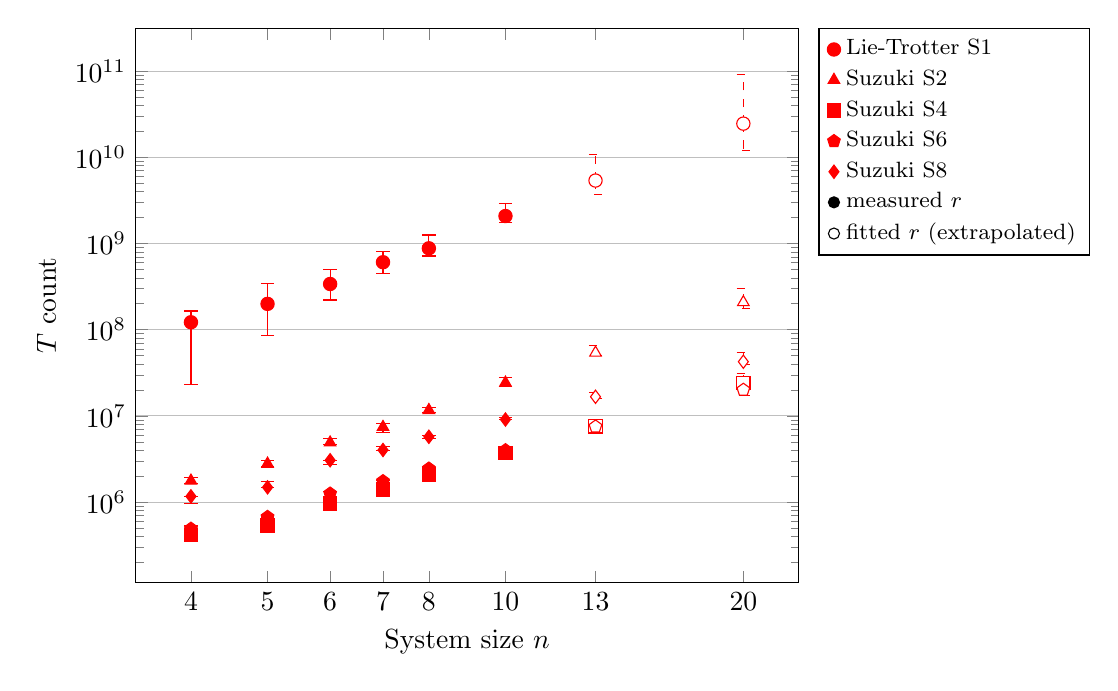
\begin{tikzpicture}
  \begin{loglogaxis}[
    width=10cm,
    xlabel={System size $n$},
    ylabel={$T$ count},
    xtick={4,5,6,7,8,10,13,20},
    xticklabels={4,5,6,7,8,10,13,20},
    ymajorgrids=true,
    legend pos=outer north east,
    legend cell align=left,
    legend style={font=\footnotesize},
  ]
    \addplot[only marks, red, mark=*, mark size=2.4pt, mark options={solid, fill=red}, error bars/.cd, y dir=both, y explicit, error bar style={red}] coordinates {
      (4,122032132) += (0,43012412) -= (0,98964458)
      (5,199402167) += (0,141546483) -= (0,114415587)
      (6,339047007) += (0,166002525) -= (0,117870207)
      (7,606237382) += (0,204620666) -= (0,155004910)
      (8,879209894) += (0,377799882) -= (0,162092340)
      (10,2082317356) += (0,862076772) -= (0,344145796)
    };
    \addlegendentry{Lie-Trotter S1}
    \addplot[only marks, red, mark=*, mark size=2.4pt, mark options={solid, fill=white}, forget plot, error bars/.cd, y dir=both, y explicit, error bar style={red, dashed}] coordinates {
      (13,5375044845) += (0,5310027219) -= (0,1702392705)
      (20,24572872883) += (0,66858476181) -= (0,12697597343)
    };
    \addplot[only marks, red, mark=triangle*, mark size=2.4pt, mark options={solid, fill=red}, error bars/.cd, y dir=both, y explicit, error bar style={red}] coordinates {
      (4,1770918) += (0,147882) -= (0,145186)
      (5,2788988) += (0,226588) -= (0,232918)
      (6,4900920) += (0,623180) -= (0,259036)
      (7,7419156) += (0,797708) -= (0,1059272)
      (8,11673189) += (0,947219) -= (0,761365)
      (10,24258489) += (0,3492291) -= (0,2298411)
    };
    \addlegendentry{Suzuki S2}
    \addplot[only marks, red, mark=triangle*, mark size=2.4pt, mark options={solid, fill=white}, forget plot, error bars/.cd, y dir=both, y explicit, error bar style={red, dashed}] coordinates {
      (13,54054476) += (0,12119840) -= (0,4232192)
      (20,208003079) += (0,94302923) -= (0,31889559)
    };
    \addplot[only marks, red, mark=square*, mark size=2.4pt, mark options={solid, fill=red}, error bars/.cd, y dir=both, y explicit, error bar style={red}] coordinates {
      (4,412976) += (0,1636) -= (0,14760)
      (5,535040) += (0,32200) -= (0,18800)
      (6,944950) += (0,72670) -= (0,49600)
      (7,1401914) += (0,62182) -= (0,84474)
      (8,2059726) += (0,70194) -= (0,107298)
      (10,3733848) += (0,423458) -= (0,39068)
    };
    \addlegendentry{Suzuki S4}
    \addplot[only marks, red, mark=square*, mark size=2.4pt, mark options={solid, fill=white}, forget plot, error bars/.cd, y dir=both, y explicit, error bar style={red, dashed}] coordinates {
      (13,7564669) += (0,1247087) -= (0,436653)
      (20,24179760) += (0,6979914) -= (0,2903274)
    };
    \addplot[only marks, red, mark=pentagon*, mark size=2.4pt, mark options={solid, fill=red}, error bars/.cd, y dir=both, y explicit, error bar style={red}] coordinates {
      (4,490685) += (0,40671) -= (0,1131)
      (5,672686) += (0,38464) -= (0,1442)
      (6,1254729) += (0,64127) -= (0,81529)
      (7,1747975) += (0,52889) -= (0,148923)
      (8,2446500) += (0,93082) -= (0,3420)
      (10,3997843) += (0,318145) -= (0,196833)
    };
    \addlegendentry{Suzuki S6}
    \addplot[only marks, red, mark=pentagon*, mark size=2.4pt, mark options={solid, fill=white}, forget plot, error bars/.cd, y dir=both, y explicit, error bar style={red, dashed}] coordinates {
      (13,7514691) += (0,974349) -= (0,801299)
      (20,20063997) += (0,4611641) -= (0,2718045)
    };
    \addplot[only marks, red, mark=diamond*, mark size=2.4pt, mark options={solid, fill=red}, error bars/.cd, y dir=both, y explicit, error bar style={red}] coordinates {
      (4,1166916) += (0,3384) -= (0,192396)
      (5,1485150) += (0,266208) -= (0,2082)
      (6,3060110) += (0,6170) -= (0,317900)
      (7,4023349) += (0,360779) -= (0,14839)
      (8,5725226) += (0,217410) -= (0,217100)
      (10,9084018) += (0,580614) -= (0,10982)
    };
    \addlegendentry{Suzuki S8}
    \addplot[only marks, red, mark=diamond*, mark size=2.4pt, mark options={solid, fill=white}, forget plot, error bars/.cd, y dir=both, y explicit, error bar style={red, dashed}] coordinates {
      (13,16670469) += (0,2093523) -= (0,729797)
      (20,42551241) += (0,11351927) -= (0,3129601)
    };
    \addlegendimage{only marks, black, mark=*}
    \addlegendentry{measured $r$}
    \addlegendimage{only marks, black, mark=*, mark options={fill=white}}
    \addlegendentry{fitted $r$ (extrapolated)}
  \end{loglogaxis}
\end{tikzpicture}

\clearpage

\section*{\texttt{t/B-order4-by-formula.tex}}
Every order-4 formula at measured r; median over seeds, bars min-max\par\medskip
% Generated by plsimcount.pfseeds -- do not edit; regenerate instead.
% figure: B-order4-by-formula -- Every order-4 formula at measured r; median over seeds [1, 2, 3, 4, 5, 6, 7, 8, 9, 10], bars = min..max
% metric=t gatebase=ct merged
% seed 1: git_commit=01d3c275ceae2840002bd1aaea68f59b987c4975 git_dirty=False
% seed 2: git_commit=01d3c275ceae2840002bd1aaea68f59b987c4975 git_dirty=False
% seed 3: git_commit=01d3c275ceae2840002bd1aaea68f59b987c4975 git_dirty=False
% seed 4: git_commit=01d3c275ceae2840002bd1aaea68f59b987c4975 git_dirty=False
% seed 5: git_commit=01d3c275ceae2840002bd1aaea68f59b987c4975 git_dirty=False
% seed 6: git_commit=01d3c275ceae2840002bd1aaea68f59b987c4975 git_dirty=False
% seed 7: git_commit=01d3c275ceae2840002bd1aaea68f59b987c4975 git_dirty=False
% seed 8: git_commit=01d3c275ceae2840002bd1aaea68f59b987c4975 git_dirty=False
% seed 9: git_commit=01d3c275ceae2840002bd1aaea68f59b987c4975 git_dirty=False
% seed 10: git_commit=01d3c275ceae2840002bd1aaea68f59b987c4975 git_dirty=False
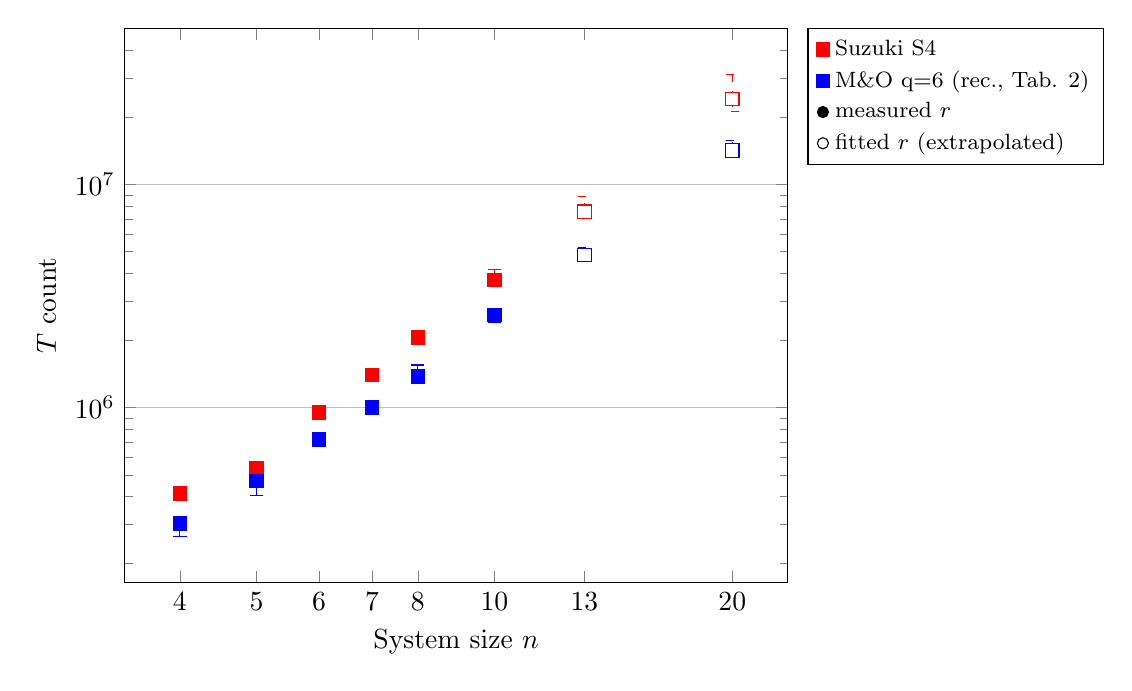
\begin{tikzpicture}
  \begin{loglogaxis}[
    width=10cm,
    xlabel={System size $n$},
    ylabel={$T$ count},
    xtick={4,5,6,7,8,10,13,20},
    xticklabels={4,5,6,7,8,10,13,20},
    ymajorgrids=true,
    legend pos=outer north east,
    legend cell align=left,
    legend style={font=\footnotesize},
  ]
    \addplot[only marks, red, mark=square*, mark size=2.4pt, mark options={solid, fill=red}, error bars/.cd, y dir=both, y explicit, error bar style={red}] coordinates {
      (4,412976) += (0,1636) -= (0,14760)
      (5,535040) += (0,32200) -= (0,18800)
      (6,944950) += (0,72670) -= (0,49600)
      (7,1401914) += (0,62182) -= (0,84474)
      (8,2059726) += (0,70194) -= (0,107298)
      (10,3733848) += (0,423458) -= (0,39068)
    };
    \addlegendentry{Suzuki S4}
    \addplot[only marks, red, mark=square*, mark size=2.4pt, mark options={solid, fill=white}, forget plot, error bars/.cd, y dir=both, y explicit, error bar style={red, dashed}] coordinates {
      (13,7564669) += (0,1247087) -= (0,436653)
      (20,24179760) += (0,6979914) -= (0,2903274)
    };
    \addplot[only marks, blue, mark=square*, mark size=2.4pt, mark options={solid, fill=blue}, error bars/.cd, y dir=both, y explicit, error bar style={blue}] coordinates {
      (4,302600) += (0,12120) -= (0,38120)
      (5,468630) += (0,10674) -= (0,63054)
      (6,721242) += (0,23090) -= (0,43082)
      (7,1002051) += (0,56097) -= (0,61363)
      (8,1379246) += (0,175790) -= (0,69022)
      (10,2604576) += (0,120480) -= (0,205344)
    };
    \addlegendentry{M\&O q=6 (rec., Tab. 2)}
    \addplot[only marks, blue, mark=square*, mark size=2.4pt, mark options={solid, fill=white}, forget plot, error bars/.cd, y dir=both, y explicit, error bar style={blue, dashed}] coordinates {
      (13,4828267) += (0,393873) -= (0,149249)
      (20,14213266) += (0,1487930) -= (0,810202)
    };
    \addlegendimage{only marks, black, mark=*}
    \addlegendentry{measured $r$}
    \addlegendimage{only marks, black, mark=*, mark options={fill=white}}
    \addlegendentry{fitted $r$ (extrapolated)}
  \end{loglogaxis}
\end{tikzpicture}

\clearpage

\section*{\texttt{t/B-order6-by-formula.tex}}
Every order-6 formula at measured r; median over seeds, bars min-max\par\medskip
% Generated by pysimcount.pfseeds -- do not edit; regenerate instead.
% figure: B-order6-by-formula -- Every order-6 formula at measured r; median over seeds [1, 2, 3, 4, 5, 6, 7, 8, 9, 10], bars = min..max
% metric=t gatebase=ct merged
% seed 1: git_commit=01d3c275ceae2840002bd1aaea68f59b987c4975 git_dirty=False
% seed 2: git_commit=01d3c275ceae2840002bd1aaea68f59b987c4975 git_dirty=False
% seed 3: git_commit=01d3c275ceae2840002bd1aaea68f59b987c4975 git_dirty=False
% seed 4: git_commit=01d3c275ceae2840002bd1aaea68f59b987c4975 git_dirty=False
% seed 5: git_commit=01d3c275ceae2840002bd1aaea68f59b987c4975 git_dirty=False
% seed 6: git_commit=01d3c275ceae2840002bd1aaea68f59b987c4975 git_dirty=False
% seed 7: git_commit=01d3c275ceae2840002bd1aaea68f59b987c4975 git_dirty=False
% seed 8: git_commit=01d3c275ceae2840002bd1aaea68f59b987c4975 git_dirty=False
% seed 9: git_commit=01d3c275ceae2840002bd1aaea68f59b987c4975 git_dirty=False
% seed 10: git_commit=01d3c275ceae2840002bd1aaea68f59b987c4975 git_dirty=False
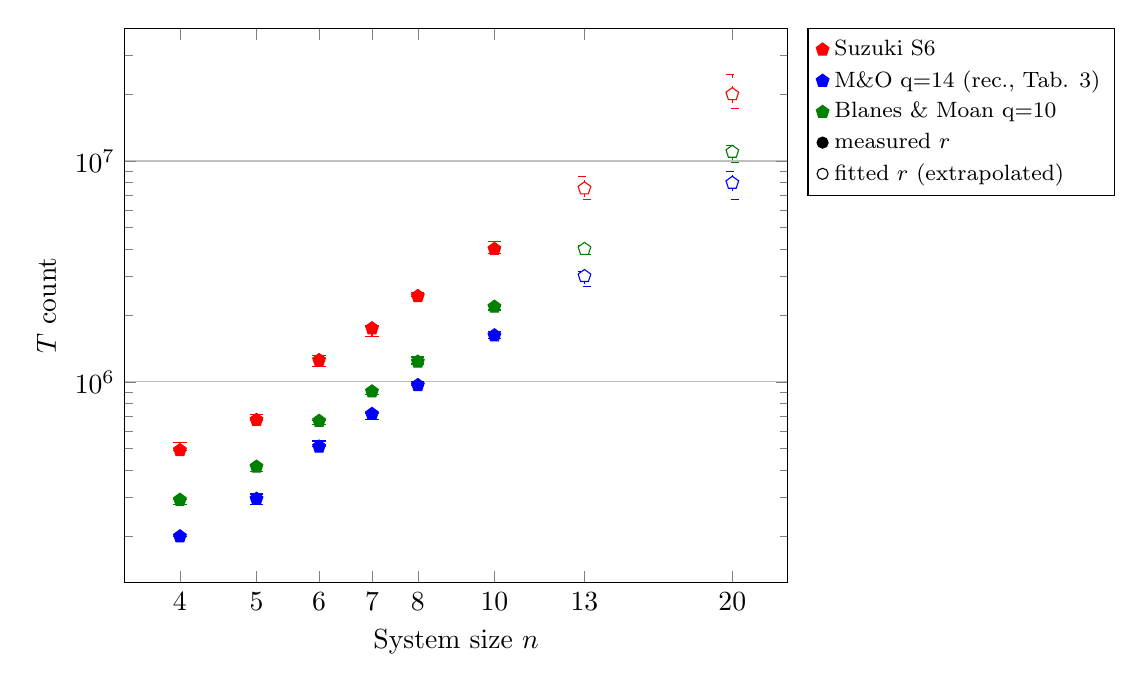
\begin{tikzpicture}
  \begin{loglogaxis}[
    width=10cm,
    xlabel={System size $n$},
    ylabel={$T$ count},
    xtick={4,5,6,7,8,10,13,20},
    xticklabels={4,5,6,7,8,10,13,20},
    ymajorgrids=true,
    legend pos=outer north east,
    legend cell align=left,
    legend style={font=\footnotesize},
  ]
    \addplot[only marks, red, mark=pentagon*, mark size=2.4pt, mark options={solid, fill=red}, error bars/.cd, y dir=both, y explicit, error bar style={red}] coordinates {
      (4,490685) += (0,40671) -= (0,1131)
      (5,672686) += (0,38464) -= (0,1442)
      (6,1254729) += (0,64127) -= (0,81529)
      (7,1747975) += (0,52889) -= (0,148923)
      (8,2446500) += (0,93082) -= (0,3420)
      (10,3997843) += (0,318145) -= (0,196833)
    };
    \addlegendentry{Suzuki S6}
    \addplot[only marks, red, mark=pentagon*, mark size=2.4pt, mark options={solid, fill=white}, forget plot, error bars/.cd, y dir=both, y explicit, error bar style={red, dashed}] coordinates {
      (13,7514691) += (0,974349) -= (0,801299)
      (20,20063997) += (0,4611641) -= (0,2718045)
    };
    \addplot[only marks, blue, mark=pentagon*, mark size=2.4pt, mark options={solid, fill=blue}, error bars/.cd, y dir=both, y explicit, error bar style={blue}] coordinates {
      (4,199740) += (0,60) -= (0,380)
      (5,295424) += (0,15496) -= (0,15672)
      (6,509056) += (0,30728) -= (0,1152)
      (7,715540) += (0,874) -= (0,40504)
      (8,966548) += (0,41496) -= (0,924)
      (10,1624174) += (0,64346) -= (0,53038)
    };
    \addlegendentry{M\&O q=14 (rec., Tab. 3)}
    \addplot[only marks, blue, mark=pentagon*, mark size=2.4pt, mark options={solid, fill=white}, forget plot, error bars/.cd, y dir=both, y explicit, error bar style={blue, dashed}] coordinates {
      (13,3012480) += (0,162468) -= (0,309312)
      (20,7963132) += (0,983748) -= (0,1234620)
    };
    \addplot[only marks, green!50!black, mark=pentagon*, mark size=2.4pt, mark options={solid, fill=green!50!black}, error bars/.cd, y dir=both, y explicit, error bar style={green!50!black}] coordinates {
      (4,292400) += (0,800) -= (0,13784)
      (5,413028) += (0,484) -= (0,20874)
      (6,665550) += (0,1102) -= (0,24126)
      (7,904662) += (0,19118) -= (0,28118)
      (8,1234038) += (0,61890) -= (0,28222)
      (10,2187862) += (0,28082) -= (0,70838)
    };
    \addlegendentry{Blanes \& Moan q=10}
    \addplot[only marks, green!50!black, mark=pentagon*, mark size=2.4pt, mark options={solid, fill=white}, forget plot, error bars/.cd, y dir=both, y explicit, error bar style={green!50!black, dashed}] coordinates {
      (13,3998210) += (0,160390) -= (0,224462)
      (20,10999812) += (0,781452) -= (0,1141124)
    };
    \addlegendimage{only marks, black, mark=*}
    \addlegendentry{measured $r$}
    \addlegendimage{only marks, black, mark=*, mark options={fill=white}}
    \addlegendentry{fitted $r$ (extrapolated)}
  \end{loglogaxis}
\end{tikzpicture}

\clearpage

\section*{\texttt{t/B-order8-by-formula.tex}}
Every order-8 formula at measured r; median over seeds, bars min-max\par\medskip
% Generated by pysimcount.pfseeds -- do not edit; regenerate instead.
% figure: B-order8-by-formula -- Every order-8 formula at measured r; median over seeds [1, 2, 3, 4, 5, 6, 7, 8, 9, 10], bars = min..max
% metric=t gatebase=ct merged
% seed 1: git_commit=01d3c275ceae2840002bd1aaea68f59b987c4975 git_dirty=False
% seed 2: git_commit=01d3c275ceae2840002bd1aaea68f59b987c4975 git_dirty=False
% seed 3: git_commit=01d3c275ceae2840002bd1aaea68f59b987c4975 git_dirty=False
% seed 4: git_commit=01d3c275ceae2840002bd1aaea68f59b987c4975 git_dirty=False
% seed 5: git_commit=01d3c275ceae2840002bd1aaea68f59b987c4975 git_dirty=False
% seed 6: git_commit=01d3c275ceae2840002bd1aaea68f59b987c4975 git_dirty=False
% seed 7: git_commit=01d3c275ceae2840002bd1aaea68f59b987c4975 git_dirty=False
% seed 8: git_commit=01d3c275ceae2840002bd1aaea68f59b987c4975 git_dirty=False
% seed 9: git_commit=01d3c275ceae2840002bd1aaea68f59b987c4975 git_dirty=False
% seed 10: git_commit=01d3c275ceae2840002bd1aaea68f59b987c4975 git_dirty=False
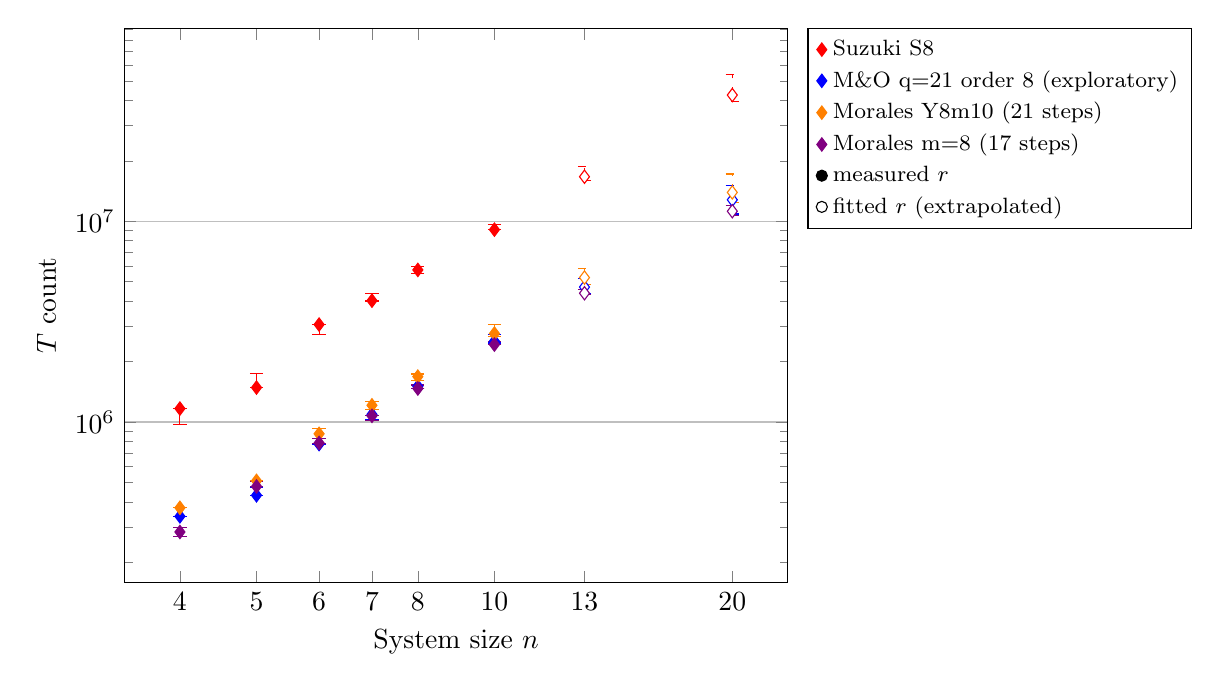
\begin{tikzpicture}
  \begin{loglogaxis}[
    width=10cm,
    xlabel={System size $n$},
    ylabel={$T$ count},
    xtick={4,5,6,7,8,10,13,20},
    xticklabels={4,5,6,7,8,10,13,20},
    ymajorgrids=true,
    legend pos=outer north east,
    legend cell align=left,
    legend style={font=\footnotesize},
  ]
    \addplot[only marks, red, mark=diamond*, mark size=2.4pt, mark options={solid, fill=red}, error bars/.cd, y dir=both, y explicit, error bar style={red}] coordinates {
      (4,1166916) += (0,3384) -= (0,192396)
      (5,1485150) += (0,266208) -= (0,2082)
      (6,3060110) += (0,6170) -= (0,317900)
      (7,4023349) += (0,360779) -= (0,14839)
      (8,5725226) += (0,217410) -= (0,217100)
      (10,9084018) += (0,580614) -= (0,10982)
    };
    \addlegendentry{Suzuki S8}
    \addplot[only marks, red, mark=diamond*, mark size=2.4pt, mark options={solid, fill=white}, forget plot, error bars/.cd, y dir=both, y explicit, error bar style={red, dashed}] coordinates {
      (13,16670469) += (0,2093523) -= (0,729797)
      (20,42551241) += (0,11351927) -= (0,3129601)
    };
    \addplot[only marks, blue, mark=diamond*, mark size=2.4pt, mark options={solid, fill=blue}, error bars/.cd, y dir=both, y explicit, error bar style={blue}] coordinates {
      (4,338998) += (0,792) -= (0,550)
      (5,431486) += (0,42202) -= (0,726)
      (6,776512) += (0,49892) -= (0,1504)
      (7,1091664) += (0,68376) -= (0,63504)
      (8,1506077) += (0,35751) -= (0,34937)
      (10,2527798) += (0,199114) -= (0,50502)
    };
    \addlegendentry{M\&O q=21 order 8 (exploratory)}
    \addplot[only marks, blue, mark=diamond*, mark size=2.4pt, mark options={solid, fill=white}, forget plot, error bars/.cd, y dir=both, y explicit, error bar style={blue, dashed}] coordinates {
      (13,4702618) += (0,486062) -= (0,335430)
      (20,12795346) += (0,2221934) -= (0,1927074)
    };
    \addplot[only marks, orange, mark=diamond*, mark size=2.4pt, mark options={solid, fill=orange}, error bars/.cd, y dir=both, y explicit, error bar style={orange}] coordinates {
      (4,373908) += (0,324) -= (0,420)
      (5,509288) += (0,624) -= (0,468)
      (6,873450) += (0,53180) -= (0,48338)
      (7,1211994) += (0,55162) -= (0,59074)
      (8,1683875) += (0,50585) -= (0,79043)
      (10,2759488) += (0,295802) -= (0,95534)
    };
    \addlegendentry{Morales Y8m10 (21 steps)}
    \addplot[only marks, orange, mark=diamond*, mark size=2.4pt, mark options={solid, fill=white}, forget plot, error bars/.cd, y dir=both, y explicit, error bar style={orange, dashed}] coordinates {
      (13,5244750) += (0,585450) -= (0,387282)
      (20,13925864) += (0,3288788) -= (0,1482490)
    };
    \addplot[only marks, violet, mark=diamond*, mark size=2.4pt, mark options={solid, fill=violet}, error bars/.cd, y dir=both, y explicit, error bar style={violet}] coordinates {
      (4,283369) += (0,15191) -= (0,14661)
      (5,477480) += (0,30360) -= (0,1500)
      (6,786680) += (0,42820) -= (0,960)
      (7,1073295) += (0,1495) -= (0,56543)
      (8,1469043) += (0,60765) -= (0,1215)
      (10,2430855) += (0,81441) -= (0,3535)
    };
    \addlegendentry{Morales m=8 (17 steps)}
    \addplot[only marks, violet, mark=diamond*, mark size=2.4pt, mark options={solid, fill=white}, forget plot, error bars/.cd, y dir=both, y explicit, error bar style={violet, dashed}] coordinates {
      (13,4381387) += (0,171399) -= (0,78087)
      (20,11224575) += (0,782625) -= (0,527147)
    };
    \addlegendimage{only marks, black, mark=*}
    \addlegendentry{measured $r$}
    \addlegendimage{only marks, black, mark=*, mark options={fill=white}}
    \addlegendentry{fitted $r$ (extrapolated)}
  \end{loglogaxis}
\end{tikzpicture}

\clearpage

\section*{\texttt{t/B-all-by-formula.tex}}
Every formula at measured r; median over seeds, bars min-max\par\medskip
% Generated by plsimcount.pfseeds -- do not edit; regenerate instead.
% figure: B-all-by-formula -- Every formula at measured r; median over seeds [1, 2, 3, 4, 5, 6, 7, 8, 9, 10], bars = min..max
% metric=t gatebase=ct merged
% seed 1: git_commit=01d3c275ceae2840002bd1aaea68f59b987c4975 git_dirty=False
% seed 2: git_commit=01d3c275ceae2840002bd1aaea68f59b987c4975 git_dirty=False
% seed 3: git_commit=01d3c275ceae2840002bd1aaea68f59b987c4975 git_dirty=False
% seed 4: git_commit=01d3c275ceae2840002bd1aaea68f59b987c4975 git_dirty=False
% seed 5: git_commit=01d3c275ceae2840002bd1aaea68f59b987c4975 git_dirty=False
% seed 6: git_commit=01d3c275ceae2840002bd1aaea68f59b987c4975 git_dirty=False
% seed 7: git_commit=01d3c275ceae2840002bd1aaea68f59b987c4975 git_dirty=False
% seed 8: git_commit=01d3c275ceae2840002bd1aaea68f59b987c4975 git_dirty=False
% seed 9: git_commit=01d3c275ceae2840002bd1aaea68f59b987c4975 git_dirty=False
% seed 10: git_commit=01d3c275ceae2840002bd1aaea68f59b987c4975 git_dirty=False
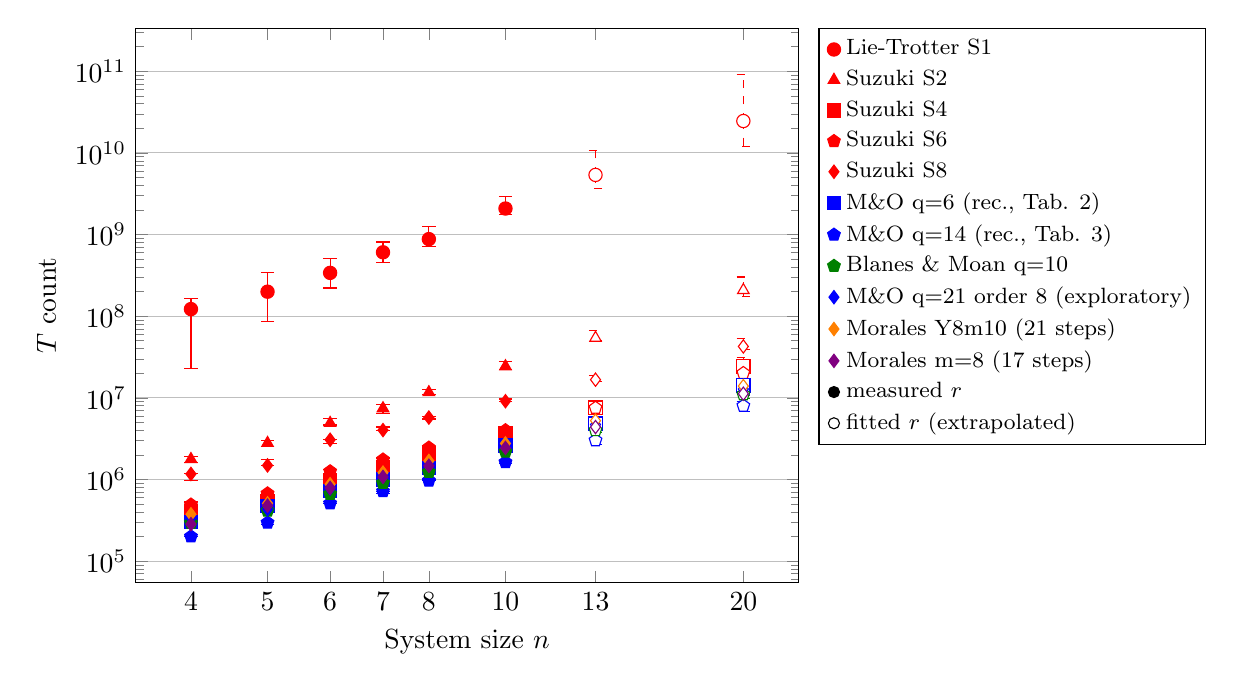
\begin{tikzpicture}
  \begin{loglogaxis}[
    width=10cm,
    xlabel={System size $n$},
    ylabel={$T$ count},
    xtick={4,5,6,7,8,10,13,20},
    xticklabels={4,5,6,7,8,10,13,20},
    ymajorgrids=true,
    legend pos=outer north east,
    legend cell align=left,
    legend style={font=\footnotesize},
  ]
    \addplot[only marks, red, mark=*, mark size=2.4pt, mark options={solid, fill=red}, error bars/.cd, y dir=both, y explicit, error bar style={red}] coordinates {
      (4,122032132) += (0,43012412) -= (0,98964458)
      (5,199402167) += (0,141546483) -= (0,114415587)
      (6,339047007) += (0,166002525) -= (0,117870207)
      (7,606237382) += (0,204620666) -= (0,155004910)
      (8,879209894) += (0,377799882) -= (0,162092340)
      (10,2082317356) += (0,862076772) -= (0,344145796)
    };
    \addlegendentry{Lie-Trotter S1}
    \addplot[only marks, red, mark=*, mark size=2.4pt, mark options={solid, fill=white}, forget plot, error bars/.cd, y dir=both, y explicit, error bar style={red, dashed}] coordinates {
      (13,5375044845) += (0,5310027219) -= (0,1702392705)
      (20,24572872883) += (0,66858476181) -= (0,12697597343)
    };
    \addplot[only marks, red, mark=triangle*, mark size=2.4pt, mark options={solid, fill=red}, error bars/.cd, y dir=both, y explicit, error bar style={red}] coordinates {
      (4,1770918) += (0,147882) -= (0,145186)
      (5,2788988) += (0,226588) -= (0,232918)
      (6,4900920) += (0,623180) -= (0,259036)
      (7,7419156) += (0,797708) -= (0,1059272)
      (8,11673189) += (0,947219) -= (0,761365)
      (10,24258489) += (0,3492291) -= (0,2298411)
    };
    \addlegendentry{Suzuki S2}
    \addplot[only marks, red, mark=triangle*, mark size=2.4pt, mark options={solid, fill=white}, forget plot, error bars/.cd, y dir=both, y explicit, error bar style={red, dashed}] coordinates {
      (13,54054476) += (0,12119840) -= (0,4232192)
      (20,208003079) += (0,94302923) -= (0,31889559)
    };
    \addplot[only marks, red, mark=square*, mark size=2.4pt, mark options={solid, fill=red}, error bars/.cd, y dir=both, y explicit, error bar style={red}] coordinates {
      (4,412976) += (0,1636) -= (0,14760)
      (5,535040) += (0,32200) -= (0,18800)
      (6,944950) += (0,72670) -= (0,49600)
      (7,1401914) += (0,62182) -= (0,84474)
      (8,2059726) += (0,70194) -= (0,107298)
      (10,3733848) += (0,423458) -= (0,39068)
    };
    \addlegendentry{Suzuki S4}
    \addplot[only marks, red, mark=square*, mark size=2.4pt, mark options={solid, fill=white}, forget plot, error bars/.cd, y dir=both, y explicit, error bar style={red, dashed}] coordinates {
      (13,7564669) += (0,1247087) -= (0,436653)
      (20,24179760) += (0,6979914) -= (0,2903274)
    };
    \addplot[only marks, red, mark=pentagon*, mark size=2.4pt, mark options={solid, fill=red}, error bars/.cd, y dir=both, y explicit, error bar style={red}] coordinates {
      (4,490685) += (0,40671) -= (0,1131)
      (5,672686) += (0,38464) -= (0,1442)
      (6,1254729) += (0,64127) -= (0,81529)
      (7,1747975) += (0,52889) -= (0,148923)
      (8,2446500) += (0,93082) -= (0,3420)
      (10,3997843) += (0,318145) -= (0,196833)
    };
    \addlegendentry{Suzuki S6}
    \addplot[only marks, red, mark=pentagon*, mark size=2.4pt, mark options={solid, fill=white}, forget plot, error bars/.cd, y dir=both, y explicit, error bar style={red, dashed}] coordinates {
      (13,7514691) += (0,974349) -= (0,801299)
      (20,20063997) += (0,4611641) -= (0,2718045)
    };
    \addplot[only marks, red, mark=diamond*, mark size=2.4pt, mark options={solid, fill=red}, error bars/.cd, y dir=both, y explicit, error bar style={red}] coordinates {
      (4,1166916) += (0,3384) -= (0,192396)
      (5,1485150) += (0,266208) -= (0,2082)
      (6,3060110) += (0,6170) -= (0,317900)
      (7,4023349) += (0,360779) -= (0,14839)
      (8,5725226) += (0,217410) -= (0,217100)
      (10,9084018) += (0,580614) -= (0,10982)
    };
    \addlegendentry{Suzuki S8}
    \addplot[only marks, red, mark=diamond*, mark size=2.4pt, mark options={solid, fill=white}, forget plot, error bars/.cd, y dir=both, y explicit, error bar style={red, dashed}] coordinates {
      (13,16670469) += (0,2093523) -= (0,729797)
      (20,42551241) += (0,11351927) -= (0,3129601)
    };
    \addplot[only marks, blue, mark=square*, mark size=2.4pt, mark options={solid, fill=blue}, error bars/.cd, y dir=both, y explicit, error bar style={blue}] coordinates {
      (4,302600) += (0,12120) -= (0,38120)
      (5,468630) += (0,10674) -= (0,63054)
      (6,721242) += (0,23090) -= (0,43082)
      (7,1002051) += (0,56097) -= (0,61363)
      (8,1379246) += (0,175790) -= (0,69022)
      (10,2604576) += (0,120480) -= (0,205344)
    };
    \addlegendentry{M\&O q=6 (rec., Tab. 2)}
    \addplot[only marks, blue, mark=square*, mark size=2.4pt, mark options={solid, fill=white}, forget plot, error bars/.cd, y dir=both, y explicit, error bar style={blue, dashed}] coordinates {
      (13,4828267) += (0,393873) -= (0,149249)
      (20,14213266) += (0,1487930) -= (0,810202)
    };
    \addplot[only marks, blue, mark=pentagon*, mark size=2.4pt, mark options={solid, fill=blue}, error bars/.cd, y dir=both, y explicit, error bar style={blue}] coordinates {
      (4,199740) += (0,60) -= (0,380)
      (5,295424) += (0,15496) -= (0,15672)
      (6,509056) += (0,30728) -= (0,1152)
      (7,715540) += (0,874) -= (0,40504)
      (8,966548) += (0,41496) -= (0,924)
      (10,1624174) += (0,64346) -= (0,53038)
    };
    \addlegendentry{M\&O q=14 (rec., Tab. 3)}
    \addplot[only marks, blue, mark=pentagon*, mark size=2.4pt, mark options={solid, fill=white}, forget plot, error bars/.cd, y dir=both, y explicit, error bar style={blue, dashed}] coordinates {
      (13,3012480) += (0,162468) -= (0,309312)
      (20,7963132) += (0,983748) -= (0,1234620)
    };
    \addplot[only marks, green!50!black, mark=pentagon*, mark size=2.4pt, mark options={solid, fill=green!50!black}, error bars/.cd, y dir=both, y explicit, error bar style={green!50!black}] coordinates {
      (4,292400) += (0,800) -= (0,13784)
      (5,413028) += (0,484) -= (0,20874)
      (6,665550) += (0,1102) -= (0,24126)
      (7,904662) += (0,19118) -= (0,28118)
      (8,1234038) += (0,61890) -= (0,28222)
      (10,2187862) += (0,28082) -= (0,70838)
    };
    \addlegendentry{Blanes \& Moan q=10}
    \addplot[only marks, green!50!black, mark=pentagon*, mark size=2.4pt, mark options={solid, fill=white}, forget plot, error bars/.cd, y dir=both, y explicit, error bar style={green!50!black, dashed}] coordinates {
      (13,3998210) += (0,160390) -= (0,224462)
      (20,10999812) += (0,781452) -= (0,1141124)
    };
    \addplot[only marks, blue, mark=diamond*, mark size=2.4pt, mark options={solid, fill=blue}, error bars/.cd, y dir=both, y explicit, error bar style={blue}] coordinates {
      (4,338998) += (0,792) -= (0,550)
      (5,431486) += (0,42202) -= (0,726)
      (6,776512) += (0,49892) -= (0,1504)
      (7,1091664) += (0,68376) -= (0,63504)
      (8,1506077) += (0,35751) -= (0,34937)
      (10,2527798) += (0,199114) -= (0,50502)
    };
    \addlegendentry{M\&O q=21 order 8 (exploratory)}
    \addplot[only marks, blue, mark=diamond*, mark size=2.4pt, mark options={solid, fill=white}, forget plot, error bars/.cd, y dir=both, y explicit, error bar style={blue, dashed}] coordinates {
      (13,4702618) += (0,486062) -= (0,335430)
      (20,12795346) += (0,2221934) -= (0,1927074)
    };
    \addplot[only marks, orange, mark=diamond*, mark size=2.4pt, mark options={solid, fill=orange}, error bars/.cd, y dir=both, y explicit, error bar style={orange}] coordinates {
      (4,373908) += (0,324) -= (0,420)
      (5,509288) += (0,624) -= (0,468)
      (6,873450) += (0,53180) -= (0,48338)
      (7,1211994) += (0,55162) -= (0,59074)
      (8,1683875) += (0,50585) -= (0,79043)
      (10,2759488) += (0,295802) -= (0,95534)
    };
    \addlegendentry{Morales Y8m10 (21 steps)}
    \addplot[only marks, orange, mark=diamond*, mark size=2.4pt, mark options={solid, fill=white}, forget plot, error bars/.cd, y dir=both, y explicit, error bar style={orange, dashed}] coordinates {
      (13,5244750) += (0,585450) -= (0,387282)
      (20,13925864) += (0,3288788) -= (0,1482490)
    };
    \addplot[only marks, violet, mark=diamond*, mark size=2.4pt, mark options={solid, fill=violet}, error bars/.cd, y dir=both, y explicit, error bar style={violet}] coordinates {
      (4,283369) += (0,15191) -= (0,14661)
      (5,477480) += (0,30360) -= (0,1500)
      (6,786680) += (0,42820) -= (0,960)
      (7,1073295) += (0,1495) -= (0,56543)
      (8,1469043) += (0,60765) -= (0,1215)
      (10,2430855) += (0,81441) -= (0,3535)
    };
    \addlegendentry{Morales m=8 (17 steps)}
    \addplot[only marks, violet, mark=diamond*, mark size=2.4pt, mark options={solid, fill=white}, forget plot, error bars/.cd, y dir=both, y explicit, error bar style={violet, dashed}] coordinates {
      (13,4381387) += (0,171399) -= (0,78087)
      (20,11224575) += (0,782625) -= (0,527147)
    };
    \addlegendimage{only marks, black, mark=*}
    \addlegendentry{measured $r$}
    \addlegendimage{only marks, black, mark=*, mark options={fill=white}}
    \addlegendentry{fitted $r$ (extrapolated)}
  \end{loglogaxis}
\end{tikzpicture}

\clearpage

\section*{\texttt{total/A-measured-by-order.tex}}
Suzuki formulas of each order, r from: Measured $r$; median over seeds, bars min-max\par\medskip
% Generated by pysimcount.pfseeds -- do not edit; regenerate instead.
% figure: A-measured-by-order -- Suzuki formulas of each order, r from: Measured $r$; median over seeds [1, 2, 3, 4, 5, 6, 7, 8, 9, 10], bars = min..max
% metric=total gatebase=cz merged
% seed 1: git_commit=01d3c275ceae2840002bd1aaea68f59b987c4975 git_dirty=False
% seed 2: git_commit=01d3c275ceae2840002bd1aaea68f59b987c4975 git_dirty=False
% seed 3: git_commit=01d3c275ceae2840002bd1aaea68f59b987c4975 git_dirty=False
% seed 4: git_commit=01d3c275ceae2840002bd1aaea68f59b987c4975 git_dirty=False
% seed 5: git_commit=01d3c275ceae2840002bd1aaea68f59b987c4975 git_dirty=False
% seed 6: git_commit=01d3c275ceae2840002bd1aaea68f59b987c4975 git_dirty=False
% seed 7: git_commit=01d3c275ceae2840002bd1aaea68f59b987c4975 git_dirty=False
% seed 8: git_commit=01d3c275ceae2840002bd1aaea68f59b987c4975 git_dirty=False
% seed 9: git_commit=01d3c275ceae2840002bd1aaea68f59b987c4975 git_dirty=False
% seed 10: git_commit=01d3c275ceae2840002bd1aaea68f59b987c4975 git_dirty=False
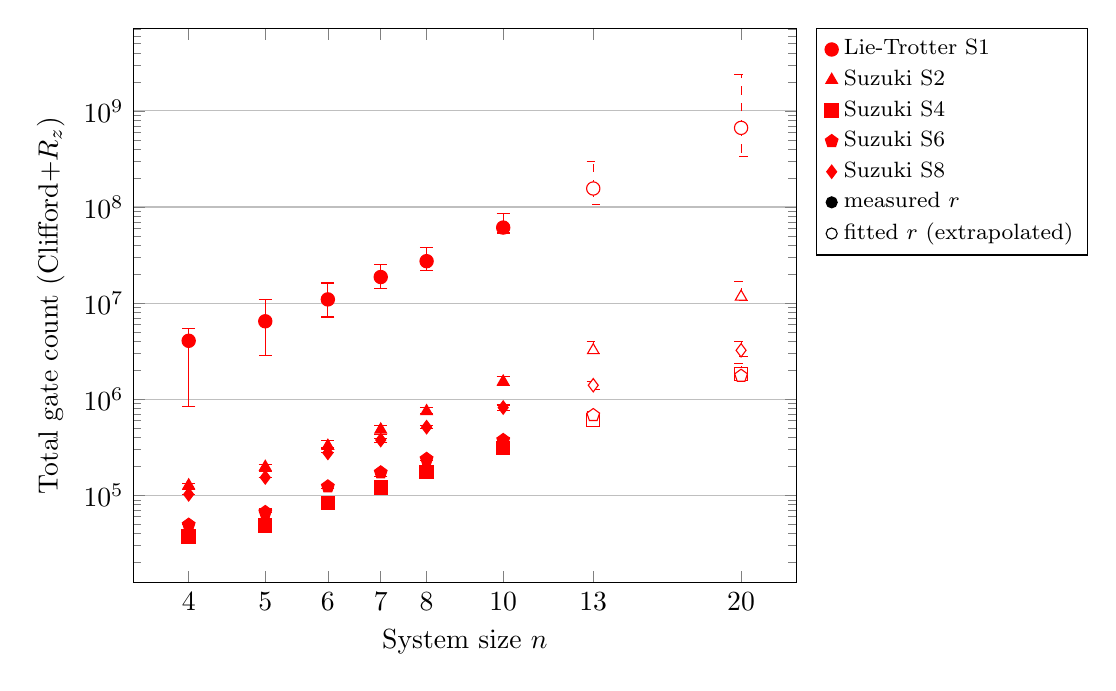
\begin{tikzpicture}
  \begin{loglogaxis}[
    width=10cm,
    xlabel={System size $n$},
    ylabel={Total gate count (Clifford+$R_z$)},
    xtick={4,5,6,7,8,10,13,20},
    xticklabels={4,5,6,7,8,10,13,20},
    ymajorgrids=true,
    legend pos=outer north east,
    legend cell align=left,
    legend style={font=\footnotesize},
  ]
    \addplot[only marks, red, mark=*, mark size=2.4pt, mark options={solid, fill=red}, error bars/.cd, y dir=both, y explicit, error bar style={red}] coordinates {
      (4,4062136) += (0,1411488) -= (0,3228472)
      (5,6480825) += (0,4436575) -= (0,3600025)
      (6,10941840) += (0,5296356) -= (0,3753360)
      (7,18715424) += (0,6624072) -= (0,4347798)
      (8,27344304) += (0,10570768) -= (0,5317104)
      (10,61189570) += (0,24481210) -= (0,7465250)
    };
    \addlegendentry{Lie-Trotter S1}
    \addplot[only marks, red, mark=*, mark size=2.4pt, mark options={solid, fill=white}, forget plot, error bars/.cd, y dir=both, y explicit, error bar style={red, dashed}] coordinates {
      (13,155918893) += (0,143251667) -= (0,49372505)
      (20,666237780) += (0,1729653900) -= (0,329848220)
    };
    \addplot[only marks, red, mark=triangle*, mark size=2.4pt, mark options={solid, fill=red}, error bars/.cd, y dir=both, y explicit, error bar style={red}] coordinates {
      (4,127008) += (0,7200) -= (0,11040)
      (5,197760) += (0,13200) -= (0,20400)
      (6,327600) += (0,49104) -= (0,15120)
      (7,483672) += (0,45864) -= (0,52584)
      (8,750912) += (0,64320) -= (0,40128)
      (10,1524720) += (0,208080) -= (0,126960)
    };
    \addlegendentry{Suzuki S2}
    \addplot[only marks, red, mark=triangle*, mark size=2.4pt, mark options={solid, fill=white}, forget plot, error bars/.cd, y dir=both, y explicit, error bar style={red, dashed}] coordinates {
      (13,3234192) += (0,718224) -= (0,222768)
      (20,11655360) += (0,5156160) -= (0,1104000)
    };
    \addplot[only marks, red, mark=square*, mark size=2.4pt, mark options={solid, fill=red}, error bars/.cd, y dir=both, y explicit, error bar style={red}] coordinates {
      (4,37312) += (0,848) -= (0,0)
      (5,48760) += (0,2120) -= (0,1060)
      (6,83952) += (0,6360) -= (0,3816)
      (7,120946) += (0,11130) -= (0,6678)
      (8,174688) += (0,6784) -= (0,6784)
      (10,310580) += (0,28620) -= (0,7420)
    };
    \addlegendentry{Suzuki S4}
    \addplot[only marks, red, mark=square*, mark size=2.4pt, mark options={solid, fill=white}, forget plot, error bars/.cd, y dir=both, y explicit, error bar style={red, dashed}] coordinates {
      (13,610454) += (0,86814) -= (0,39962)
      (20,1835920) += (0,517280) -= (0,212000)
    };
    \addplot[only marks, red, mark=pentagon*, mark size=2.4pt, mark options={solid, fill=red}, error bars/.cd, y dir=both, y explicit, error bar style={red}] coordinates {
      (4,49536) += (0,0) -= (0,0)
      (5,67080) += (0,5160) -= (0,0)
      (6,123840) += (0,6192) -= (0,6192)
      (7,173376) += (0,7224) -= (0,14448)
      (8,239424) += (0,8256) -= (0,8256)
      (10,376680) += (0,25800) -= (0,15480)
    };
    \addlegendentry{Suzuki S6}
    \addplot[only marks, red, mark=pentagon*, mark size=2.4pt, mark options={solid, fill=white}, forget plot, error bars/.cd, y dir=both, y explicit, error bar style={red, dashed}] coordinates {
      (13,684216) += (0,67080) -= (0,40248)
      (20,1754400) += (0,350880) -= (0,185760)
    };
    \addplot[only marks, red, mark=diamond*, mark size=2.4pt, mark options={solid, fill=red}, error bars/.cd, y dir=both, y explicit, error bar style={red}] coordinates {
      (4,102640) += (0,0) -= (0,0)
      (5,153960) += (0,0) -= (0,0)
      (6,277128) += (0,30792) -= (0,0)
      (7,377202) += (0,17962) -= (0,17962)
      (8,513200) += (0,20528) -= (0,20528)
      (10,821120) += (0,51320) -= (0,51320)
    };
    \addlegendentry{Suzuki S8}
    \addplot[only marks, red, mark=diamond*, mark size=2.4pt, mark options={solid, fill=white}, forget plot, error bars/.cd, y dir=both, y explicit, error bar style={red, dashed}] coordinates {
      (13,1401036) += (0,133432) -= (0,133432)
      (20,3233160) += (0,769800) -= (0,461880)
    };
    \addlegendimage{only marks, black, mark=*}
    \addlegendentry{measured $r$}
    \addlegendimage{only marks, black, mark=*, mark options={fill=white}}
    \addlegendentry{fitted $r$ (extrapolated)}
  \end{loglogaxis}
\end{tikzpicture}

\clearpage

\section*{\texttt{total/B-order4-by-formula.tex}}
Every order-4 formula at measured r; median over seeds, bars min-max\par\medskip
% Generated by pysimcount.pfseeds -- do not edit; regenerate instead.
% figure: B-order4-by-formula -- Every order-4 formula at measured r; median over seeds [1, 2, 3, 4, 5, 6, 7, 8, 9, 10], bars = min..max
% metric=total gatebase=cz merged
% seed 1: git_commit=01d3c275ceae2840002bd1aaea68f59b987c4975 git_dirty=False
% seed 2: git_commit=01d3c275ceae2840002bd1aaea68f59b987c4975 git_dirty=False
% seed 3: git_commit=01d3c275ceae2840002bd1aaea68f59b987c4975 git_dirty=False
% seed 4: git_commit=01d3c275ceae2840002bd1aaea68f59b987c4975 git_dirty=False
% seed 5: git_commit=01d3c275ceae2840002bd1aaea68f59b987c4975 git_dirty=False
% seed 6: git_commit=01d3c275ceae2840002bd1aaea68f59b987c4975 git_dirty=False
% seed 7: git_commit=01d3c275ceae2840002bd1aaea68f59b987c4975 git_dirty=False
% seed 8: git_commit=01d3c275ceae2840002bd1aaea68f59b987c4975 git_dirty=False
% seed 9: git_commit=01d3c275ceae2840002bd1aaea68f59b987c4975 git_dirty=False
% seed 10: git_commit=01d3c275ceae2840002bd1aaea68f59b987c4975 git_dirty=False
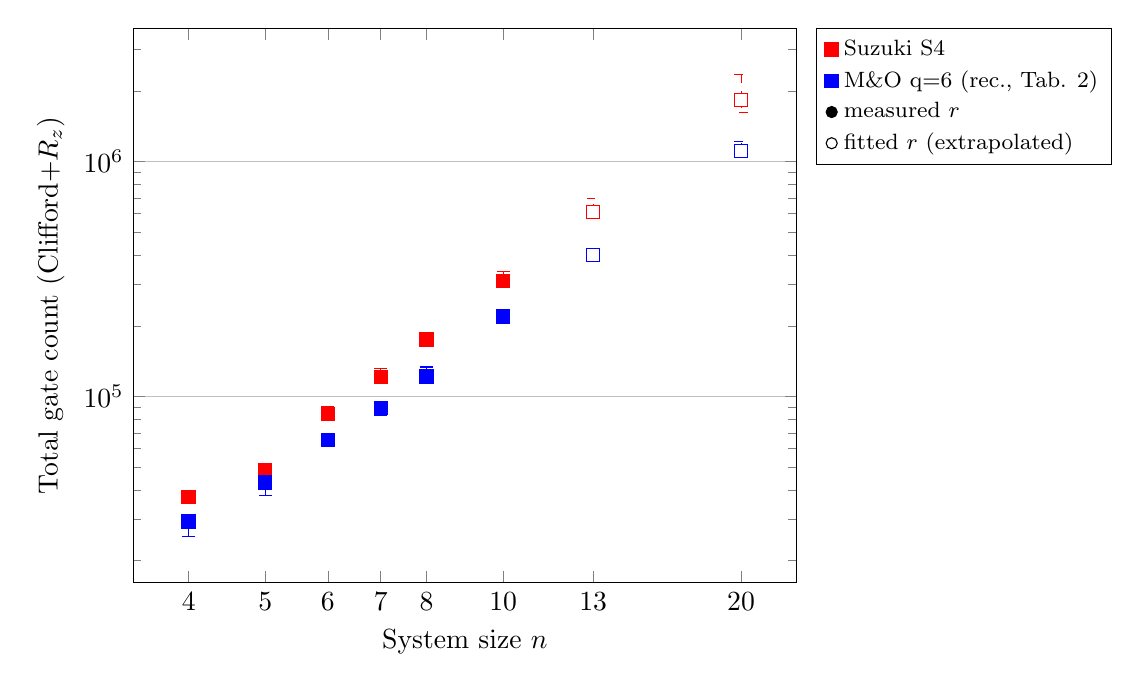
\begin{tikzpicture}
  \begin{loglogaxis}[
    width=10cm,
    xlabel={System size $n$},
    ylabel={Total gate count (Clifford+$R_z$)},
    xtick={4,5,6,7,8,10,13,20},
    xticklabels={4,5,6,7,8,10,13,20},
    ymajorgrids=true,
    legend pos=outer north east,
    legend cell align=left,
    legend style={font=\footnotesize},
  ]
    \addplot[only marks, red, mark=square*, mark size=2.4pt, mark options={solid, fill=red}, error bars/.cd, y dir=both, y explicit, error bar style={red}] coordinates {
      (4,37312) += (0,848) -= (0,0)
      (5,48760) += (0,2120) -= (0,1060)
      (6,83952) += (0,6360) -= (0,3816)
      (7,120946) += (0,11130) -= (0,6678)
      (8,174688) += (0,6784) -= (0,6784)
      (10,310580) += (0,28620) -= (0,7420)
    };
    \addlegendentry{Suzuki S4}
    \addplot[only marks, red, mark=square*, mark size=2.4pt, mark options={solid, fill=white}, forget plot, error bars/.cd, y dir=both, y explicit, error bar style={red, dashed}] coordinates {
      (13,610454) += (0,86814) -= (0,39962)
      (20,1835920) += (0,517280) -= (0,212000)
    };
    \addplot[only marks, blue, mark=square*, mark size=2.4pt, mark options={solid, fill=blue}, error bars/.cd, y dir=both, y explicit, error bar style={blue}] coordinates {
      (4,29348) += (0,1012) -= (0,4048)
      (5,43010) += (0,1265) -= (0,5060)
      (6,65274) += (0,1518) -= (0,3036)
      (7,89436) += (0,4428) -= (0,6198)
      (8,121440) += (0,12144) -= (0,6072)
      (10,218845) += (0,8855) -= (0,13915)
    };
    \addlegendentry{M\&O q=6 (rec., Tab. 2)}
    \addplot[only marks, blue, mark=square*, mark size=2.4pt, mark options={solid, fill=white}, forget plot, error bars/.cd, y dir=both, y explicit, error bar style={blue, dashed}] coordinates {
      (13,399614) += (0,27956) -= (0,8222)
      (20,1110670) += (0,108790) -= (0,43010)
    };
    \addlegendimage{only marks, black, mark=*}
    \addlegendentry{measured $r$}
    \addlegendimage{only marks, black, mark=*, mark options={fill=white}}
    \addlegendentry{fitted $r$ (extrapolated)}
  \end{loglogaxis}
\end{tikzpicture}

\clearpage

\section*{\texttt{total/B-order6-by-formula.tex}}
Every order-6 formula at measured r; median over seeds, bars min-max\par\medskip
% Generated by plsimcount.pfseeds -- do not edit; regenerate instead.
% figure: B-order6-by-formula -- Every order-6 formula at measured r; median over seeds [1, 2, 3, 4, 5, 6, 7, 8, 9, 10], bars = min..max
% metric=total gatebase=cz merged
% seed 1: git_commit=01d3c275ceae2840002bd1aaea68f59b987c4975 git_dirty=False
% seed 2: git_commit=01d3c275ceae2840002bd1aaea68f59b987c4975 git_dirty=False
% seed 3: git_commit=01d3c275ceae2840002bd1aaea68f59b987c4975 git_dirty=False
% seed 4: git_commit=01d3c275ceae2840002bd1aaea68f59b987c4975 git_dirty=False
% seed 5: git_commit=01d3c275ceae2840002bd1aaea68f59b987c4975 git_dirty=False
% seed 6: git_commit=01d3c275ceae2840002bd1aaea68f59b987c4975 git_dirty=False
% seed 7: git_commit=01d3c275ceae2840002bd1aaea68f59b987c4975 git_dirty=False
% seed 8: git_commit=01d3c275ceae2840002bd1aaea68f59b987c4975 git_dirty=False
% seed 9: git_commit=01d3c275ceae2840002bd1aaea68f59b987c4975 git_dirty=False
% seed 10: git_commit=01d3c275ceae2840002bd1aaea68f59b987c4975 git_dirty=False
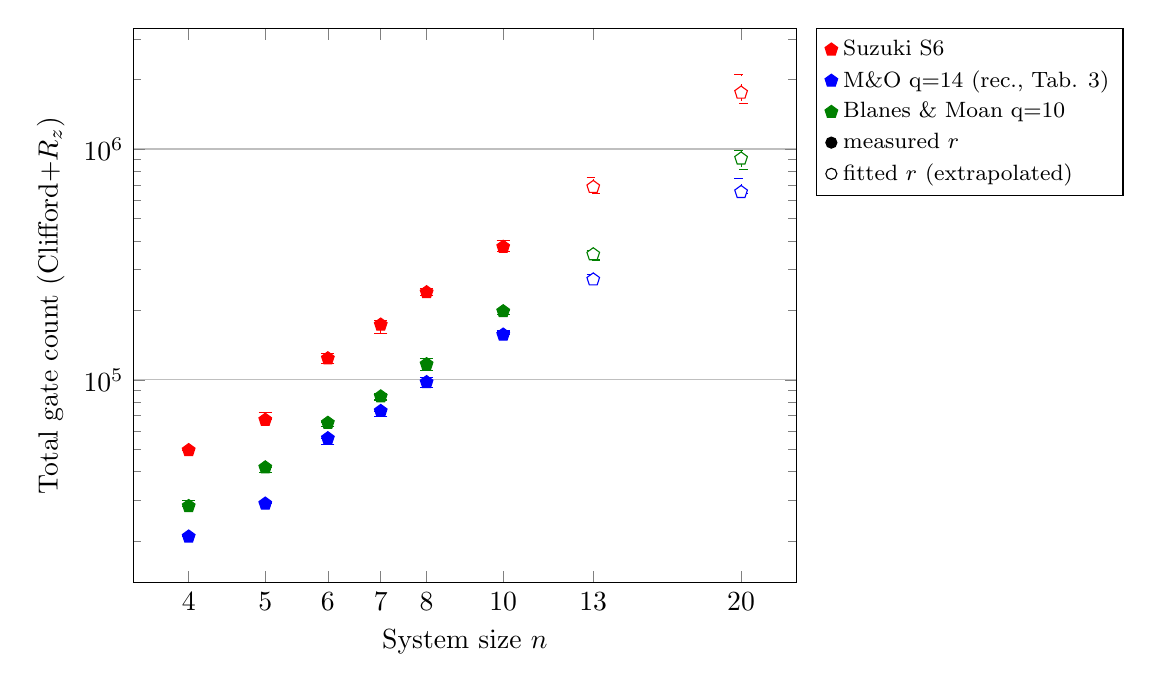
\begin{tikzpicture}
  \begin{loglogaxis}[
    width=10cm,
    xlabel={System size $n$},
    ylabel={Total gate count (Clifford+$R_z$)},
    xtick={4,5,6,7,8,10,13,20},
    xticklabels={4,5,6,7,8,10,13,20},
    ymajorgrids=true,
    legend pos=outer north east,
    legend cell align=left,
    legend style={font=\footnotesize},
  ]
    \addplot[only marks, red, mark=pentagon*, mark size=2.4pt, mark options={solid, fill=red}, error bars/.cd, y dir=both, y explicit, error bar style={red}] coordinates {
      (4,49536) += (0,0) -= (0,0)
      (5,67080) += (0,5160) -= (0,0)
      (6,123840) += (0,6192) -= (0,6192)
      (7,173376) += (0,7224) -= (0,14448)
      (8,239424) += (0,8256) -= (0,8256)
      (10,376680) += (0,25800) -= (0,15480)
    };
    \addlegendentry{Suzuki S6}
    \addplot[only marks, red, mark=pentagon*, mark size=2.4pt, mark options={solid, fill=white}, forget plot, error bars/.cd, y dir=both, y explicit, error bar style={red, dashed}] coordinates {
      (13,684216) += (0,67080) -= (0,40248)
      (20,1754400) += (0,350880) -= (0,185760)
    };
    \addplot[only marks, blue, mark=pentagon*, mark size=2.4pt, mark options={solid, fill=blue}, error bars/.cd, y dir=both, y explicit, error bar style={blue}] coordinates {
      (4,20916) += (0,0) -= (0,0)
      (5,29050) += (0,0) -= (0,0)
      (6,55776) += (0,0) -= (0,3486)
      (7,73206) += (0,0) -= (0,4067)
      (8,97608) += (0,4648) -= (0,4648)
      (10,156870) += (0,5810) -= (0,0)
    };
    \addlegendentry{M\&O q=14 (rec., Tab. 3)}
    \addplot[only marks, blue, mark=pentagon*, mark size=2.4pt, mark options={solid, fill=white}, forget plot, error bars/.cd, y dir=both, y explicit, error bar style={blue, dashed}] coordinates {
      (13,271908) += (0,15106) -= (0,0)
      (20,650720) += (0,92960) -= (0,11620)
    };
    \addplot[only marks, green!50!black, mark=pentagon*, mark size=2.4pt, mark options={solid, fill=green!50!black}, error bars/.cd, y dir=both, y explicit, error bar style={green!50!black}] coordinates {
      (4,28356) += (0,1668) -= (0,0)
      (5,41700) += (0,0) -= (0,2085)
      (6,65052) += (0,0) -= (0,2502)
      (7,84651) += (0,2919) -= (0,2919)
      (8,116760) += (0,6672) -= (0,6672)
      (10,198075) += (0,2085) -= (0,6255)
    };
    \addlegendentry{Blanes \& Moan q=10}
    \addplot[only marks, green!50!black, mark=pentagon*, mark size=2.4pt, mark options={solid, fill=white}, forget plot, error bars/.cd, y dir=both, y explicit, error bar style={green!50!black, dashed}] coordinates {
      (13,349654) += (0,13552) -= (0,18974)
      (20,909060) += (0,75060) -= (0,91740)
    };
    \addlegendimage{only marks, black, mark=*}
    \addlegendentry{measured $r$}
    \addlegendimage{only marks, black, mark=*, mark options={fill=white}}
    \addlegendentry{fitted $r$ (extrapolated)}
  \end{loglogaxis}
\end{tikzpicture}

\clearpage

\section*{\texttt{total/B-order8-by-formula.tex}}
Every order-8 formula at measured r; median over seeds, bars min-max\par\medskip
% Generated by plsimcount.pfseeds -- do not edit; regenerate instead.
% figure: B-order8-by-formula -- Every order-8 formula at measured r; median over seeds [1, 2, 3, 4, 5, 6, 7, 8, 9, 10], bars = min..max
% metric=total gatebase=cz merged
% seed 1: git_commit=01d3c275ceae2840002bd1aaea68f59b987c4975 git_dirty=False
% seed 2: git_commit=01d3c275ceae2840002bd1aaea68f59b987c4975 git_dirty=False
% seed 3: git_commit=01d3c275ceae2840002bd1aaea68f59b987c4975 git_dirty=False
% seed 4: git_commit=01d3c275ceae2840002bd1aaea68f59b987c4975 git_dirty=False
% seed 5: git_commit=01d3c275ceae2840002bd1aaea68f59b987c4975 git_dirty=False
% seed 6: git_commit=01d3c275ceae2840002bd1aaea68f59b987c4975 git_dirty=False
% seed 7: git_commit=01d3c275ceae2840002bd1aaea68f59b987c4975 git_dirty=False
% seed 8: git_commit=01d3c275ceae2840002bd1aaea68f59b987c4975 git_dirty=False
% seed 9: git_commit=01d3c275ceae2840002bd1aaea68f59b987c4975 git_dirty=False
% seed 10: git_commit=01d3c275ceae2840002bd1aaea68f59b987c4975 git_dirty=False
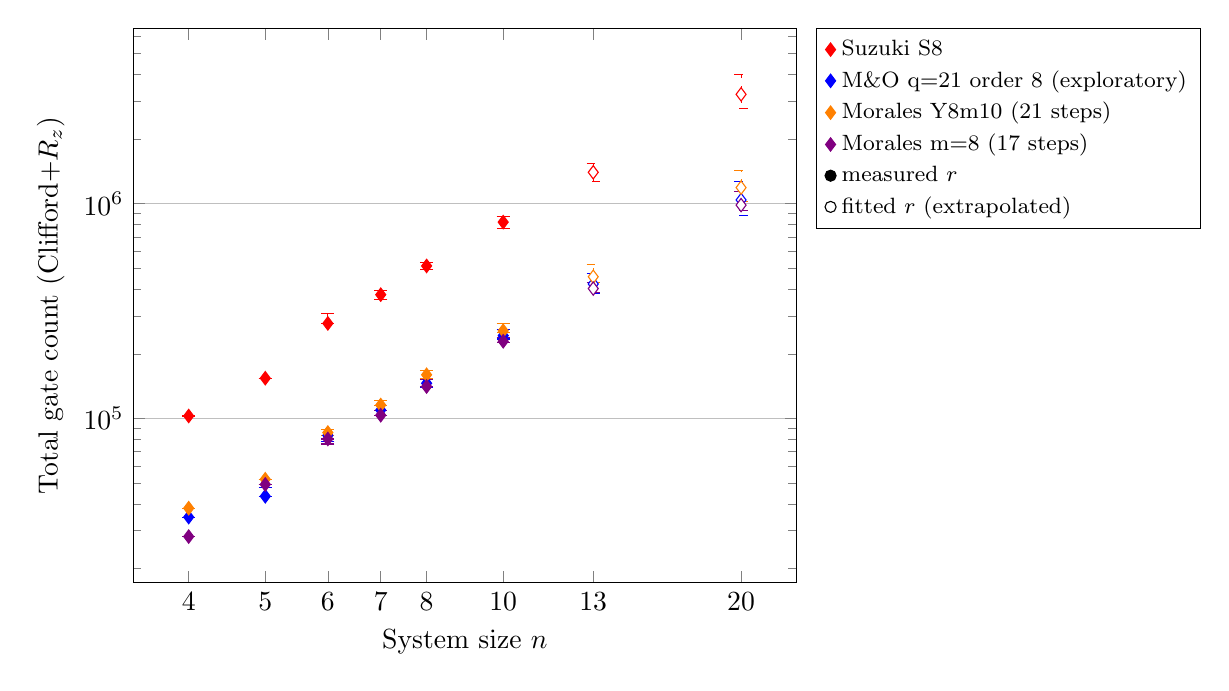
\begin{tikzpicture}
  \begin{loglogaxis}[
    width=10cm,
    xlabel={System size $n$},
    ylabel={Total gate count (Clifford+$R_z$)},
    xtick={4,5,6,7,8,10,13,20},
    xticklabels={4,5,6,7,8,10,13,20},
    ymajorgrids=true,
    legend pos=outer north east,
    legend cell align=left,
    legend style={font=\footnotesize},
  ]
    \addplot[only marks, red, mark=diamond*, mark size=2.4pt, mark options={solid, fill=red}, error bars/.cd, y dir=both, y explicit, error bar style={red}] coordinates {
      (4,102640) += (0,0) -= (0,0)
      (5,153960) += (0,0) -= (0,0)
      (6,277128) += (0,30792) -= (0,0)
      (7,377202) += (0,17962) -= (0,17962)
      (8,513200) += (0,20528) -= (0,20528)
      (10,821120) += (0,51320) -= (0,51320)
    };
    \addlegendentry{Suzuki S8}
    \addplot[only marks, red, mark=diamond*, mark size=2.4pt, mark options={solid, fill=white}, forget plot, error bars/.cd, y dir=both, y explicit, error bar style={red, dashed}] coordinates {
      (13,1401036) += (0,133432) -= (0,133432)
      (20,3233160) += (0,769800) -= (0,461880)
    };
    \addplot[only marks, blue, mark=diamond*, mark size=2.4pt, mark options={solid, fill=blue}, error bars/.cd, y dir=both, y explicit, error bar style={blue}] coordinates {
      (4,34720) += (0,0) -= (0,0)
      (5,43400) += (0,4340) -= (0,0)
      (6,83328) += (0,5208) -= (0,5208)
      (7,109368) += (0,6076) -= (0,6076)
      (8,145824) += (0,6944) -= (0,6944)
      (10,243040) += (0,17360) -= (0,8680)
    };
    \addlegendentry{M\&O q=21 order 8 (exploratory)}
    \addplot[only marks, blue, mark=diamond*, mark size=2.4pt, mark options={solid, fill=white}, forget plot, error bars/.cd, y dir=both, y explicit, error bar style={blue, dashed}] coordinates {
      (13,423150) += (0,50778) -= (0,39494)
      (20,1041600) += (0,225680) -= (0,156240)
    };
    \addplot[only marks, orange, mark=diamond*, mark size=2.4pt, mark options={solid, fill=orange}, error bars/.cd, y dir=both, y explicit, error bar style={orange}] coordinates {
      (4,38192) += (0,0) -= (0,0)
      (5,52080) += (0,0) -= (0,0)
      (6,85932) += (0,2604) -= (0,2604)
      (7,115444) += (0,6076) -= (0,0)
      (8,159712) += (0,6944) -= (0,6944)
      (10,256060) += (0,21700) -= (0,4340)
    };
    \addlegendentry{Morales Y8m10 (21 steps)}
    \addplot[only marks, orange, mark=diamond*, mark size=2.4pt, mark options={solid, fill=white}, forget plot, error bars/.cd, y dir=both, y explicit, error bar style={orange, dashed}] coordinates {
      (13,457002) += (0,62062) -= (0,28210)
      (20,1189160) += (0,234360) -= (0,164920)
    };
    \addplot[only marks, violet, mark=diamond*, mark size=2.4pt, mark options={solid, fill=violet}, error bars/.cd, y dir=both, y explicit, error bar style={violet}] coordinates {
      (4,28160) += (0,0) -= (0,0)
      (5,49280) += (0,0) -= (0,0)
      (6,80256) += (0,0) -= (0,4224)
      (7,103488) += (0,4928) -= (0,0)
      (8,140800) += (0,11264) -= (0,0)
      (10,228800) += (0,10560) -= (0,3520)
    };
    \addlegendentry{Morales m=8 (17 steps)}
    \addplot[only marks, violet, mark=diamond*, mark size=2.4pt, mark options={solid, fill=white}, forget plot, error bars/.cd, y dir=both, y explicit, error bar style={violet, dashed}] coordinates {
      (13,402688) += (0,27456) -= (0,18304)
      (20,985600) += (0,154880) -= (0,56320)
    };
    \addlegendimage{only marks, black, mark=*}
    \addlegendentry{measured $r$}
    \addlegendimage{only marks, black, mark=*, mark options={fill=white}}
    \addlegendentry{fitted $r$ (extrapolated)}
  \end{loglogaxis}
\end{tikzpicture}

\clearpage

\section*{\texttt{total/B-all-by-formula.tex}}
Every formula at measured r; median over seeds, bars min-max\par\medskip
% Generated by plsimcount.pfseeds -- do not edit; regenerate instead.
% figure: B-all-by-formula -- Every formula at measured r; median over seeds [1, 2, 3, 4, 5, 6, 7, 8, 9, 10], bars = min..max
% metric=total gatebase=cz merged
% seed 1: git_commit=01d3c275ceae2840002bd1aaea68f59b987c4975 git_dirty=False
% seed 2: git_commit=01d3c275ceae2840002bd1aaea68f59b987c4975 git_dirty=False
% seed 3: git_commit=01d3c275ceae2840002bd1aaea68f59b987c4975 git_dirty=False
% seed 4: git_commit=01d3c275ceae2840002bd1aaea68f59b987c4975 git_dirty=False
% seed 5: git_commit=01d3c275ceae2840002bd1aaea68f59b987c4975 git_dirty=False
% seed 6: git_commit=01d3c275ceae2840002bd1aaea68f59b987c4975 git_dirty=False
% seed 7: git_commit=01d3c275ceae2840002bd1aaea68f59b987c4975 git_dirty=False
% seed 8: git_commit=01d3c275ceae2840002bd1aaea68f59b987c4975 git_dirty=False
% seed 9: git_commit=01d3c275ceae2840002bd1aaea68f59b987c4975 git_dirty=False
% seed 10: git_commit=01d3c275ceae2840002bd1aaea68f59b987c4975 git_dirty=False
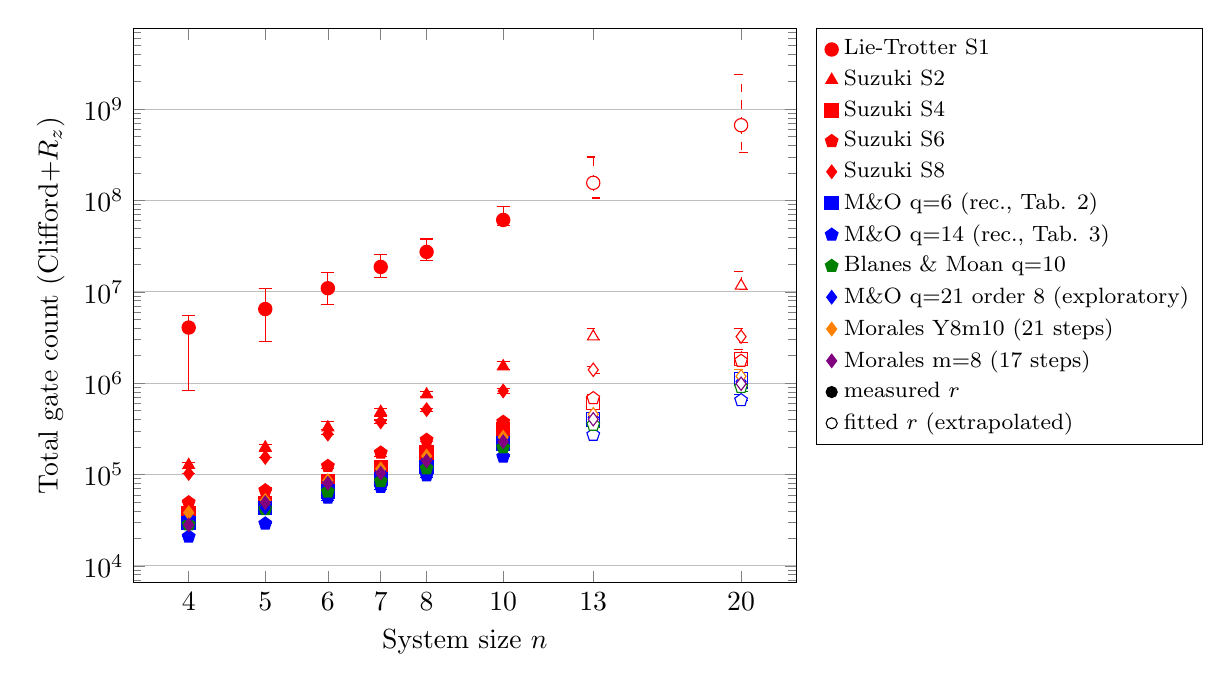
\begin{tikzpicture}
  \begin{loglogaxis}[
    width=10cm,
    xlabel={System size $n$},
    ylabel={Total gate count (Clifford+$R_z$)},
    xtick={4,5,6,7,8,10,13,20},
    xticklabels={4,5,6,7,8,10,13,20},
    ymajorgrids=true,
    legend pos=outer north east,
    legend cell align=left,
    legend style={font=\footnotesize},
  ]
    \addplot[only marks, red, mark=*, mark size=2.4pt, mark options={solid, fill=red}, error bars/.cd, y dir=both, y explicit, error bar style={red}] coordinates {
      (4,4062136) += (0,1411488) -= (0,3228472)
      (5,6480825) += (0,4436575) -= (0,3600025)
      (6,10941840) += (0,5296356) -= (0,3753360)
      (7,18715424) += (0,6624072) -= (0,4347798)
      (8,27344304) += (0,10570768) -= (0,5317104)
      (10,61189570) += (0,24481210) -= (0,7465250)
    };
    \addlegendentry{Lie-Trotter S1}
    \addplot[only marks, red, mark=*, mark size=2.4pt, mark options={solid, fill=white}, forget plot, error bars/.cd, y dir=both, y explicit, error bar style={red, dashed}] coordinates {
      (13,155918893) += (0,143251667) -= (0,49372505)
      (20,666237780) += (0,1729653900) -= (0,329848220)
    };
    \addplot[only marks, red, mark=triangle*, mark size=2.4pt, mark options={solid, fill=red}, error bars/.cd, y dir=both, y explicit, error bar style={red}] coordinates {
      (4,127008) += (0,7200) -= (0,11040)
      (5,197760) += (0,13200) -= (0,20400)
      (6,327600) += (0,49104) -= (0,15120)
      (7,483672) += (0,45864) -= (0,52584)
      (8,750912) += (0,64320) -= (0,40128)
      (10,1524720) += (0,208080) -= (0,126960)
    };
    \addlegendentry{Suzuki S2}
    \addplot[only marks, red, mark=triangle*, mark size=2.4pt, mark options={solid, fill=white}, forget plot, error bars/.cd, y dir=both, y explicit, error bar style={red, dashed}] coordinates {
      (13,3234192) += (0,718224) -= (0,222768)
      (20,11655360) += (0,5156160) -= (0,1104000)
    };
    \addplot[only marks, red, mark=square*, mark size=2.4pt, mark options={solid, fill=red}, error bars/.cd, y dir=both, y explicit, error bar style={red}] coordinates {
      (4,37312) += (0,848) -= (0,0)
      (5,48760) += (0,2120) -= (0,1060)
      (6,83952) += (0,6360) -= (0,3816)
      (7,120946) += (0,11130) -= (0,6678)
      (8,174688) += (0,6784) -= (0,6784)
      (10,310580) += (0,28620) -= (0,7420)
    };
    \addlegendentry{Suzuki S4}
    \addplot[only marks, red, mark=square*, mark size=2.4pt, mark options={solid, fill=white}, forget plot, error bars/.cd, y dir=both, y explicit, error bar style={red, dashed}] coordinates {
      (13,610454) += (0,86814) -= (0,39962)
      (20,1835920) += (0,517280) -= (0,212000)
    };
    \addplot[only marks, red, mark=pentagon*, mark size=2.4pt, mark options={solid, fill=red}, error bars/.cd, y dir=both, y explicit, error bar style={red}] coordinates {
      (4,49536) += (0,0) -= (0,0)
      (5,67080) += (0,5160) -= (0,0)
      (6,123840) += (0,6192) -= (0,6192)
      (7,173376) += (0,7224) -= (0,14448)
      (8,239424) += (0,8256) -= (0,8256)
      (10,376680) += (0,25800) -= (0,15480)
    };
    \addlegendentry{Suzuki S6}
    \addplot[only marks, red, mark=pentagon*, mark size=2.4pt, mark options={solid, fill=white}, forget plot, error bars/.cd, y dir=both, y explicit, error bar style={red, dashed}] coordinates {
      (13,684216) += (0,67080) -= (0,40248)
      (20,1754400) += (0,350880) -= (0,185760)
    };
    \addplot[only marks, red, mark=diamond*, mark size=2.4pt, mark options={solid, fill=red}, error bars/.cd, y dir=both, y explicit, error bar style={red}] coordinates {
      (4,102640) += (0,0) -= (0,0)
      (5,153960) += (0,0) -= (0,0)
      (6,277128) += (0,30792) -= (0,0)
      (7,377202) += (0,17962) -= (0,17962)
      (8,513200) += (0,20528) -= (0,20528)
      (10,821120) += (0,51320) -= (0,51320)
    };
    \addlegendentry{Suzuki S8}
    \addplot[only marks, red, mark=diamond*, mark size=2.4pt, mark options={solid, fill=white}, forget plot, error bars/.cd, y dir=both, y explicit, error bar style={red, dashed}] coordinates {
      (13,1401036) += (0,133432) -= (0,133432)
      (20,3233160) += (0,769800) -= (0,461880)
    };
    \addplot[only marks, blue, mark=square*, mark size=2.4pt, mark options={solid, fill=blue}, error bars/.cd, y dir=both, y explicit, error bar style={blue}] coordinates {
      (4,29348) += (0,1012) -= (0,4048)
      (5,43010) += (0,1265) -= (0,5060)
      (6,65274) += (0,1518) -= (0,3036)
      (7,89436) += (0,4428) -= (0,6198)
      (8,121440) += (0,12144) -= (0,6072)
      (10,218845) += (0,8855) -= (0,13915)
    };
    \addlegendentry{M\&O q=6 (rec., Tab. 2)}
    \addplot[only marks, blue, mark=square*, mark size=2.4pt, mark options={solid, fill=white}, forget plot, error bars/.cd, y dir=both, y explicit, error bar style={blue, dashed}] coordinates {
      (13,399614) += (0,27956) -= (0,8222)
      (20,1110670) += (0,108790) -= (0,43010)
    };
    \addplot[only marks, blue, mark=pentagon*, mark size=2.4pt, mark options={solid, fill=blue}, error bars/.cd, y dir=both, y explicit, error bar style={blue}] coordinates {
      (4,20916) += (0,0) -= (0,0)
      (5,29050) += (0,0) -= (0,0)
      (6,55776) += (0,0) -= (0,3486)
      (7,73206) += (0,0) -= (0,4067)
      (8,97608) += (0,4648) -= (0,4648)
      (10,156870) += (0,5810) -= (0,0)
    };
    \addlegendentry{M\&O q=14 (rec., Tab. 3)}
    \addplot[only marks, blue, mark=pentagon*, mark size=2.4pt, mark options={solid, fill=white}, forget plot, error bars/.cd, y dir=both, y explicit, error bar style={blue, dashed}] coordinates {
      (13,271908) += (0,15106) -= (0,0)
      (20,650720) += (0,92960) -= (0,11620)
    };
    \addplot[only marks, green!50!black, mark=pentagon*, mark size=2.4pt, mark options={solid, fill=green!50!black}, error bars/.cd, y dir=both, y explicit, error bar style={green!50!black}] coordinates {
      (4,28356) += (0,1668) -= (0,0)
      (5,41700) += (0,0) -= (0,2085)
      (6,65052) += (0,0) -= (0,2502)
      (7,84651) += (0,2919) -= (0,2919)
      (8,116760) += (0,6672) -= (0,6672)
      (10,198075) += (0,2085) -= (0,6255)
    };
    \addlegendentry{Blanes \& Moan q=10}
    \addplot[only marks, green!50!black, mark=pentagon*, mark size=2.4pt, mark options={solid, fill=white}, forget plot, error bars/.cd, y dir=both, y explicit, error bar style={green!50!black, dashed}] coordinates {
      (13,349654) += (0,13552) -= (0,18974)
      (20,909060) += (0,75060) -= (0,91740)
    };
    \addplot[only marks, blue, mark=diamond*, mark size=2.4pt, mark options={solid, fill=blue}, error bars/.cd, y dir=both, y explicit, error bar style={blue}] coordinates {
      (4,34720) += (0,0) -= (0,0)
      (5,43400) += (0,4340) -= (0,0)
      (6,83328) += (0,5208) -= (0,5208)
      (7,109368) += (0,6076) -= (0,6076)
      (8,145824) += (0,6944) -= (0,6944)
      (10,243040) += (0,17360) -= (0,8680)
    };
    \addlegendentry{M\&O q=21 order 8 (exploratory)}
    \addplot[only marks, blue, mark=diamond*, mark size=2.4pt, mark options={solid, fill=white}, forget plot, error bars/.cd, y dir=both, y explicit, error bar style={blue, dashed}] coordinates {
      (13,423150) += (0,50778) -= (0,39494)
      (20,1041600) += (0,225680) -= (0,156240)
    };
    \addplot[only marks, orange, mark=diamond*, mark size=2.4pt, mark options={solid, fill=orange}, error bars/.cd, y dir=both, y explicit, error bar style={orange}] coordinates {
      (4,38192) += (0,0) -= (0,0)
      (5,52080) += (0,0) -= (0,0)
      (6,85932) += (0,2604) -= (0,2604)
      (7,115444) += (0,6076) -= (0,0)
      (8,159712) += (0,6944) -= (0,6944)
      (10,256060) += (0,21700) -= (0,4340)
    };
    \addlegendentry{Morales Y8m10 (21 steps)}
    \addplot[only marks, orange, mark=diamond*, mark size=2.4pt, mark options={solid, fill=white}, forget plot, error bars/.cd, y dir=both, y explicit, error bar style={orange, dashed}] coordinates {
      (13,457002) += (0,62062) -= (0,28210)
      (20,1189160) += (0,234360) -= (0,164920)
    };
    \addplot[only marks, violet, mark=diamond*, mark size=2.4pt, mark options={solid, fill=violet}, error bars/.cd, y dir=both, y explicit, error bar style={violet}] coordinates {
      (4,28160) += (0,0) -= (0,0)
      (5,49280) += (0,0) -= (0,0)
      (6,80256) += (0,0) -= (0,4224)
      (7,103488) += (0,4928) -= (0,0)
      (8,140800) += (0,11264) -= (0,0)
      (10,228800) += (0,10560) -= (0,3520)
    };
    \addlegendentry{Morales m=8 (17 steps)}
    \addplot[only marks, violet, mark=diamond*, mark size=2.4pt, mark options={solid, fill=white}, forget plot, error bars/.cd, y dir=both, y explicit, error bar style={violet, dashed}] coordinates {
      (13,402688) += (0,27456) -= (0,18304)
      (20,985600) += (0,154880) -= (0,56320)
    };
    \addlegendimage{only marks, black, mark=*}
    \addlegendentry{measured $r$}
    \addlegendimage{only marks, black, mark=*, mark options={fill=white}}
    \addlegendentry{fitted $r$ (extrapolated)}
  \end{loglogaxis}
\end{tikzpicture}

\clearpage
\end{document}
